% VDE Template for EUSAR Papers
% Provided by Barbara Lang und Siegmar Lampe
% University of Bremen, January 2002
% English version by Jens Fischer
% German Aerospace Center (DLR), December 2005
% Additional modifications by Matthias Wei{\ss}
% FGAN, January 2009

%-----------------------------------------------------------------------------
% Type of publication
\documentclass[a4paper,10pt]{article}
%-----------------------------------------------------------------------------
% Other packets: Most packets may be downloaded from www.dante.de and
% "tcilatex.tex" can be found at (December 2005):
% http://www.mackichan.com/techtalk/v30/UsingFloat.htm
% Not all packets are necessarily needed:
\usepackage[T1]{fontenc}
\usepackage[latin1]{inputenc}
%\usepackage{ngerman} % in german language if required
\usepackage[nooneline,bf]{caption} % Figure descriptions from left margin
\usepackage{times}
\usepackage{multicol}
\usepackage{amsmath}
\usepackage{amssymb}
%\usepackage[dvips]{graphicx}
\usepackage{graphicx}
\usepackage{epsfig}
%\usepackage{natbib}
\usepackage{textgreek}
\usepackage{url}
\usepackage{listings}
\usepackage[usenames]{color} %Per permettere la colorazione dei caratteri 

\usepackage{listings}
\usepackage{color}
 
\definecolor{dkgreen}{rgb}{0,0.6,0}
\definecolor{gray}{rgb}{0.5,0.5,0.5}
\definecolor{mauve}{rgb}{0.58,0,0.82}
 
\lstset{ %
  language=C,	                % the language of the code
  basicstyle=\footnotesize,           % the size of the fonts that are used for the code
  numbers=left,                   % where to put the line-numbers
  numberstyle=\tiny\color{gray},  % the style that is used for the line-numbers
  stepnumber=2,                   % the step between two line-numbers. If it's 1, each line 
                                  % will be numbered
  numbersep=4pt,                  % how far the line-numbers are from the code
  backgroundcolor=\color{white},      % choose the background color. You must add \usepackage{color}
  showspaces=false,               % show spaces adding particular underscores
  showstringspaces=false,         % underline spaces within strings
  showtabs=false,                 % show tabs within strings adding particular underscores
  frame=single,                   % adds a frame around the code
  rulecolor=\color{black},        % if not set, the frame-color may be changed on line-breaks within not-black text (e.g. commens (green here))
  tabsize=2,                      % sets default tabsize to 2 spaces
  captionpos=b,                   % sets the caption-position to bottom
  breaklines=true,                % sets automatic line breaking
  breakatwhitespace=false,        % sets if automatic breaks should only happen at whitespace
  title=\lstname,                   % show the filename of files included with \lstinputlisting;
                                  % also try caption instead of title
  keywordstyle=\color{blue},          % keyword style
  commentstyle=\color{dkgreen},       % comment style
  stringstyle=\color{mauve},         % string literal style
  escapeinside={\%*}{*)},            % if you want to add LaTeX within your code
  morekeywords={*,Embryo_Cell,Embryo_Program,chprintf}  % if you want to add more keywords to the set
}

\usepackage{dirtree}

% Macros for Scientific Word 3.0 documents saved with the LaTeX filter.
%Copyright (C) 1994-97 TCI Software Research, Inc.
\typeout{TCILATEX Macros for Scientific Word 3.0 <05 August 1998>.}
\typeout{NOTICE:  This macro file is NOT proprietary and may be 
freely copied and distributed.}
%
\makeatletter
%
%%%%%%%%%%%%%%%%%%%%%%
% macros for time
\newcount\@hour\newcount\@minute\chardef\@x10\chardef\@xv60
\def\tcitime{
\def\@time{%
  \@minute\time\@hour\@minute\divide\@hour\@xv
  \ifnum\@hour<\@x 0\fi\the\@hour:%
  \multiply\@hour\@xv\advance\@minute-\@hour
  \ifnum\@minute<\@x 0\fi\the\@minute
  }}%

%%%%%%%%%%%%%%%%%%%%%%
% macro for hyperref
\@ifundefined{hyperref}{\def\hyperref#1#2#3#4{#2\ref{#4}#3}}{}

% macro for external program call
\@ifundefined{qExtProgCall}{\def\qExtProgCall#1#2#3#4#5#6{\relax}}{}
%%%%%%%%%%%%%%%%%%%%%%
%
% macros for graphics
%
\def\FILENAME#1{#1}%
%
\def\QCTOpt[#1]#2{%
  \def\QCTOptB{#1}
  \def\QCTOptA{#2}
}
\def\QCTNOpt#1{%
  \def\QCTOptA{#1}
  \let\QCTOptB\empty
}
\def\Qct{%
  \@ifnextchar[{%
    \QCTOpt}{\QCTNOpt}
}
\def\QCBOpt[#1]#2{%
  \def\QCBOptB{#1}
  \def\QCBOptA{#2}
}
\def\QCBNOpt#1{%
  \def\QCBOptA{#1}
  \let\QCBOptB\empty
}
\def\Qcb{%
  \@ifnextchar[{%
    \QCBOpt}{\QCBNOpt}
}
\def\PrepCapArgs{%
  \ifx\QCBOptA\empty
    \ifx\QCTOptA\empty
      {}%
    \else
      \ifx\QCTOptB\empty
        {\QCTOptA}%
      \else
        [\QCTOptB]{\QCTOptA}%
      \fi
    \fi
  \else
    \ifx\QCBOptA\empty
      {}%
    \else
      \ifx\QCBOptB\empty
        {\QCBOptA}%
      \else
        [\QCBOptB]{\QCBOptA}%
      \fi
    \fi
  \fi
}
\newcount\GRAPHICSTYPE
%\GRAPHICSTYPE 0 is for TurboTeX
%\GRAPHICSTYPE 1 is for DVIWindo (PostScript)
%%%(removed)%\GRAPHICSTYPE 2 is for psfig (PostScript)
\GRAPHICSTYPE=\z@
\def\GRAPHICSPS#1{%
 \ifcase\GRAPHICSTYPE%\GRAPHICSTYPE=0
   \special{ps: #1}%
 \or%\GRAPHICSTYPE=1
   \special{language "PS", include "#1"}%
%%%\or%\GRAPHICSTYPE=2
%%%  #1%
 \fi
}%
%
\def\GRAPHICSHP#1{\special{include #1}}%
%
% \graffile{ body }                                  %#1
%          { contentswidth (scalar)  }               %#2
%          { contentsheight (scalar) }               %#3
%          { vertical shift when in-line (scalar) }  %#4
\def\graffile#1#2#3#4{%
%%% \ifnum\GRAPHICSTYPE=\tw@
%%%  %Following if using psfig
%%%  \@ifundefined{psfig}{\input psfig.tex}{}%
%%%  \psfig{file=#1, height=#3, width=#2}%
%%% \else
  %Following for all others
  % JCS - added BOXTHEFRAME, see below
    \bgroup
    \leavevmode
    \@ifundefined{bbl@deactivate}{\def~{\string~}}{\activesoff}
    \raise -#4 \BOXTHEFRAME{%
        \hbox to #2{\raise #3\hbox to #2{\null #1\hfil}}}%
    \egroup
}%
%
% A box for drafts
\def\draftbox#1#2#3#4{%
 \leavevmode\raise -#4 \hbox{%
  \frame{\rlap{\protect\tiny #1}\hbox to #2%
   {\vrule height#3 width\z@ depth\z@\hfil}%
  }%
 }%
}%
%
\newcount\draft
\draft=\z@
\let\nographics=\draft
\newif\ifwasdraft
\wasdraftfalse

%  \GRAPHIC{ body }                                  %#1
%          { draft name }                            %#2
%          { contentswidth (scalar)  }               %#3
%          { contentsheight (scalar) }               %#4
%          { vertical shift when in-line (scalar) }  %#5
\def\GRAPHIC#1#2#3#4#5{%
 \ifnum\draft=\@ne\draftbox{#2}{#3}{#4}{#5}%
  \else\graffile{#1}{#3}{#4}{#5}%
  \fi
 }%
%
\def\addtoLaTeXparams#1{%
    \edef\LaTeXparams{\LaTeXparams #1}}%
%
% JCS -  added a switch BoxFrame that can 
% be set by including X in the frame params.
% If set a box is drawn around the frame.

\newif\ifBoxFrame \BoxFramefalse
\newif\ifOverFrame \OverFramefalse
\newif\ifUnderFrame \UnderFramefalse

\def\BOXTHEFRAME#1{%
   \hbox{%
      \ifBoxFrame
         \frame{#1}%
      \else
         {#1}%
      \fi
   }%
}


\def\doFRAMEparams#1{\BoxFramefalse\OverFramefalse\UnderFramefalse\readFRAMEparams#1\end}%
\def\readFRAMEparams#1{%
 \ifx#1\end%
  \let\next=\relax
  \else
  \ifx#1i\dispkind=\z@\fi
  \ifx#1d\dispkind=\@ne\fi
  \ifx#1f\dispkind=\tw@\fi
  \ifx#1t\addtoLaTeXparams{t}\fi
  \ifx#1b\addtoLaTeXparams{b}\fi
  \ifx#1p\addtoLaTeXparams{p}\fi
  \ifx#1h\addtoLaTeXparams{h}\fi
  \ifx#1X\BoxFrametrue\fi
  \ifx#1O\OverFrametrue\fi
  \ifx#1U\UnderFrametrue\fi
  \ifx#1w
    \ifnum\draft=1\wasdrafttrue\else\wasdraftfalse\fi
    \draft=\@ne
  \fi
  \let\next=\readFRAMEparams
  \fi
 \next
 }%
%
%Macro for In-line graphics object
%   \IFRAME{ contentswidth (scalar)  }               %#1
%          { contentsheight (scalar) }               %#2
%          { vertical shift when in-line (scalar) }  %#3
%          { draft name }                            %#4
%          { body }                                  %#5
%          { caption}                                %#6


\def\IFRAME#1#2#3#4#5#6{%
      \bgroup
      \let\QCTOptA\empty
      \let\QCTOptB\empty
      \let\QCBOptA\empty
      \let\QCBOptB\empty
      #6%
      \parindent=0pt%
      \leftskip=0pt
      \rightskip=0pt
      \setbox0 = \hbox{\QCBOptA}%
      \@tempdima = #1\relax
      \ifOverFrame
          % Do this later
          \typeout{This is not implemented yet}%
          \show\HELP
      \else
         \ifdim\wd0>\@tempdima
            \advance\@tempdima by \@tempdima
            \ifdim\wd0 >\@tempdima
               \textwidth=\@tempdima
               \setbox1 =\vbox{%
                  \noindent\hbox to \@tempdima{\hfill\GRAPHIC{#5}{#4}{#1}{#2}{#3}\hfill}\\%
                  \noindent\hbox to \@tempdima{\parbox[b]{\@tempdima}{\QCBOptA}}%
               }%
               \wd1=\@tempdima
            \else
               \textwidth=\wd0
               \setbox1 =\vbox{%
                 \noindent\hbox to \wd0{\hfill\GRAPHIC{#5}{#4}{#1}{#2}{#3}\hfill}\\%
                 \noindent\hbox{\QCBOptA}%
               }%
               \wd1=\wd0
            \fi
         \else
            %\show\BBB
            \ifdim\wd0>0pt
              \hsize=\@tempdima
              \setbox1 =\vbox{%
                \unskip\GRAPHIC{#5}{#4}{#1}{#2}{0pt}%
                \break
                \unskip\hbox to \@tempdima{\hfill \QCBOptA\hfill}%
              }%
              \wd1=\@tempdima
           \else
              \hsize=\@tempdima
              \setbox1 =\vbox{%
                \unskip\GRAPHIC{#5}{#4}{#1}{#2}{0pt}%
              }%
              \wd1=\@tempdima
           \fi
         \fi
         \@tempdimb=\ht1
         \advance\@tempdimb by \dp1
         \advance\@tempdimb by -#2%
         \advance\@tempdimb by #3%
         \leavevmode
         \raise -\@tempdimb \hbox{\box1}%
      \fi
      \egroup%
}%
%
%Macro for Display graphics object
%   \DFRAME{ contentswidth (scalar)  }               %#1
%          { contentsheight (scalar) }               %#2
%          { draft label }                           %#3
%          { name }                                  %#4
%          { caption}                                %#5
\def\DFRAME#1#2#3#4#5{%
 \begin{center}
     \let\QCTOptA\empty
     \let\QCTOptB\empty
     \let\QCBOptA\empty
     \let\QCBOptB\empty
     \ifOverFrame 
        #5\QCTOptA\par
     \fi
     \GRAPHIC{#4}{#3}{#1}{#2}{\z@}
     \ifUnderFrame 
        \nobreak\par\nobreak#5\QCBOptA
     \fi
 \end{center}%
 }%
%
%Macro for Floating graphic object
%   \FFRAME{ framedata f|i tbph x F|T }              %#1
%          { contentswidth (scalar)  }               %#2
%          { contentsheight (scalar) }               %#3
%          { caption }                               %#4
%          { label }                                 %#5
%          { draft name }                            %#6
%          { body }                                  %#7
\def\FFRAME#1#2#3#4#5#6#7{%
 %If float.sty loaded and float option is 'h', change to 'H'  (gp) 1998/09/05
  \@ifundefined{floatstyle}
    {%floatstyle undefined (and float.sty not present), no change
     \begin{figure}[#1]%
    }
    {%floatstyle DEFINED
	 \ifx#1h%Only the h parameter, change to H
      \begin{figure}[H]%
	 \else
      \begin{figure}[#1]%
	 \fi
	}
  \let\QCTOptA\empty
  \let\QCTOptB\empty
  \let\QCBOptA\empty
  \let\QCBOptB\empty
  \ifOverFrame
    #4
    \ifx\QCTOptA\empty
    \else
      \ifx\QCTOptB\empty
        \caption{\QCTOptA}%
      \else
        \caption[\QCTOptB]{\QCTOptA}%
      \fi
    \fi
    \ifUnderFrame\else
      \label{#5}%
    \fi
  \else
    \UnderFrametrue%
  \fi
  \begin{center}\GRAPHIC{#7}{#6}{#2}{#3}{\z@}\end{center}%
  \ifUnderFrame
    #4
    \ifx\QCBOptA\empty
      \caption{}%
    \else
      \ifx\QCBOptB\empty
        \caption{\QCBOptA}%
      \else
        \caption[\QCBOptB]{\QCBOptA}%
      \fi
    \fi
    \label{#5}%
  \fi
  \end{figure}%
 }%
%
%
%    \FRAME{ framedata f|i tbph x F|T }              %#1
%          { contentswidth (scalar)  }               %#2
%          { contentsheight (scalar) }               %#3
%          { vertical shift when in-line (scalar) }  %#4
%          { caption }                               %#5
%          { label }                                 %#6
%          { name }                                  %#7
%          { body }                                  %#8
%
%    framedata is a string which can contain the following
%    characters: idftbphxFT
%    Their meaning is as follows:
%             i, d or f : in-line, display, or floating
%             t,b,p,h   : LaTeX floating placement options
%             x         : fit contents box to contents
%             F or T    : Figure or Table. 
%                         Later this can expand
%                         to a more general float class.
%
%
\newcount\dispkind%

\def\makeactives{
  \catcode`\"=\active
  \catcode`\;=\active
  \catcode`\:=\active
  \catcode`\'=\active
  \catcode`\~=\active
}
\bgroup
   \makeactives
   \gdef\activesoff{%
      \def"{\string"}
      \def;{\string;}
      \def:{\string:}
      \def'{\string'}
      \def~{\string~}
      %\bbl@deactivate{"}%
      %\bbl@deactivate{;}%
      %\bbl@deactivate{:}%
      %\bbl@deactivate{'}%
    }
\egroup

\def\FRAME#1#2#3#4#5#6#7#8{%
 \bgroup
 \ifnum\draft=\@ne
   \wasdrafttrue
 \else
   \wasdraftfalse%
 \fi
 \def\LaTeXparams{}%
 \dispkind=\z@
 \def\LaTeXparams{}%
 \doFRAMEparams{#1}%
 \ifnum\dispkind=\z@\IFRAME{#2}{#3}{#4}{#7}{#8}{#5}\else
  \ifnum\dispkind=\@ne\DFRAME{#2}{#3}{#7}{#8}{#5}\else
   \ifnum\dispkind=\tw@
    \edef\@tempa{\noexpand\FFRAME{\LaTeXparams}}%
    \@tempa{#2}{#3}{#5}{#6}{#7}{#8}%
    \fi
   \fi
  \fi
  \ifwasdraft\draft=1\else\draft=0\fi{}%
  \egroup
 }%
%
% This macro added to let SW gobble a parameter that
% should not be passed on and expanded. 

\def\TEXUX#1{"texux"}

%
% Macros for text attributes:
%
\def\BF#1{{\bf {#1}}}%
\def\NEG#1{\leavevmode\hbox{\rlap{\thinspace/}{$#1$}}}%
%
%%%%%%%%%%%%%%%%%%%%%%%%%%%%%%%%%%%%%%%%%%%%%%%%%%%%%%%%%%%%%%%%%%%%%%%%
%
%
% macros for user - defined functions
\def\limfunc#1{\mathop{\rm #1}}%
\def\func#1{\mathop{\rm #1}\nolimits}%
% macro for unit names
\def\unit#1{\mathop{\rm #1}\nolimits}%

%
% miscellaneous 
\long\def\QQQ#1#2{%
     \long\expandafter\def\csname#1\endcsname{#2}}%
\@ifundefined{QTP}{\def\QTP#1{}}{}
\@ifundefined{QEXCLUDE}{\def\QEXCLUDE#1{}}{}
\@ifundefined{Qlb}{\def\Qlb#1{#1}}{}
\@ifundefined{Qlt}{\def\Qlt#1{#1}}{}
\def\QWE{}%
\long\def\QQA#1#2{}%
\def\QTR#1#2{{\csname#1\endcsname #2}}%(gp) Is this the best?
\long\def\TeXButton#1#2{#2}%
\long\def\QSubDoc#1#2{#2}%
\def\EXPAND#1[#2]#3{}%
\def\NOEXPAND#1[#2]#3{}%
\def\PROTECTED{}%
\def\LaTeXparent#1{}%
\def\ChildStyles#1{}%
\def\ChildDefaults#1{}%
\def\QTagDef#1#2#3{}%

% Constructs added with Scientific Notebook
\@ifundefined{correctchoice}{\def\correctchoice{\relax}}{}
\@ifundefined{HTML}{\def\HTML#1{\relax}}{}
\@ifundefined{TCIIcon}{\def\TCIIcon#1#2#3#4{\relax}}{}
\if@compatibility
  \typeout{Not defining UNICODE or CustomNote commands for LaTeX 2.09.}
\else
  \providecommand{\UNICODE}[2][]{}
  \providecommand{\CustomNote}[3][]{\marginpar{#3}}
\fi

%
% Macros for style editor docs
\@ifundefined{StyleEditBeginDoc}{\def\StyleEditBeginDoc{\relax}}{}
%
% Macros for footnotes
\def\QQfnmark#1{\footnotemark}
\def\QQfntext#1#2{\addtocounter{footnote}{#1}\footnotetext{#2}}
%
% Macros for indexing.
%
\@ifundefined{TCIMAKEINDEX}{}{\makeindex}%
%
% Attempts to avoid problems with other styles
\@ifundefined{abstract}{%
 \def\abstract{%
  \if@twocolumn
   \section*{Abstract (Not appropriate in this style!)}%
   \else \small 
   \begin{center}{\bf Abstract\vspace{-.5em}\vspace{\z@}}\end{center}%
   \quotation 
   \fi
  }%
 }{%
 }%
\@ifundefined{endabstract}{\def\endabstract
  {\if@twocolumn\else\endquotation\fi}}{}%
\@ifundefined{maketitle}{\def\maketitle#1{}}{}%
\@ifundefined{affiliation}{\def\affiliation#1{}}{}%
\@ifundefined{proof}{\def\proof{\noindent{\bfseries Proof. }}}{}%
\@ifundefined{endproof}{\def\endproof{\mbox{\ \rule{.1in}{.1in}}}}{}%
\@ifundefined{newfield}{\def\newfield#1#2{}}{}%
\@ifundefined{chapter}{\def\chapter#1{\par(Chapter head:)#1\par }%
 \newcount\c@chapter}{}%
\@ifundefined{part}{\def\part#1{\par(Part head:)#1\par }}{}%
\@ifundefined{section}{\def\section#1{\par(Section head:)#1\par }}{}%
\@ifundefined{subsection}{\def\subsection#1%
 {\par(Subsection head:)#1\par }}{}%
\@ifundefined{subsubsection}{\def\subsubsection#1%
 {\par(Subsubsection head:)#1\par }}{}%
\@ifundefined{paragraph}{\def\paragraph#1%
 {\par(Subsubsubsection head:)#1\par }}{}%
\@ifundefined{subparagraph}{\def\subparagraph#1%
 {\par(Subsubsubsubsection head:)#1\par }}{}%
%%%%%%%%%%%%%%%%%%%%%%%%%%%%%%%%%%%%%%%%%%%%%%%%%%%%%%%%%%%%%%%%%%%%%%%%
% These symbols are not recognized by LaTeX
\@ifundefined{therefore}{\def\therefore{}}{}%
\@ifundefined{backepsilon}{\def\backepsilon{}}{}%
\@ifundefined{yen}{\def\yen{\hbox{\rm\rlap=Y}}}{}%
\@ifundefined{registered}{%
   \def\registered{\relax\ifmmode{}\r@gistered
                    \else$\m@th\r@gistered$\fi}%
 \def\r@gistered{^{\ooalign
  {\hfil\raise.07ex\hbox{$\scriptstyle\rm\text{R}$}\hfil\crcr
  \mathhexbox20D}}}}{}%
\@ifundefined{Eth}{\def\Eth{}}{}%
\@ifundefined{eth}{\def\eth{}}{}%
\@ifundefined{Thorn}{\def\Thorn{}}{}%
\@ifundefined{thorn}{\def\thorn{}}{}%
% A macro to allow any symbol that requires math to appear in text
\def\TEXTsymbol#1{\mbox{$#1$}}%
\@ifundefined{degree}{\def\degree{{}^{\circ}}}{}%
%
% macros for T3TeX files
\newdimen\theight
\def\Column{%
 \vadjust{\setbox\z@=\hbox{\scriptsize\quad\quad tcol}%
  \theight=\ht\z@\advance\theight by \dp\z@\advance\theight by \lineskip
  \kern -\theight \vbox to \theight{%
   \rightline{\rlap{\box\z@}}%
   \vss
   }%
  }%
 }%
%
\def\qed{%
 \ifhmode\unskip\nobreak\fi\ifmmode\ifinner\else\hskip5\p@\fi\fi
 \hbox{\hskip5\p@\vrule width4\p@ height6\p@ depth1.5\p@\hskip\p@}%
 }%
%
\def\cents{\hbox{\rm\rlap/c}}%
\def\miss{\hbox{\vrule height2\p@ width 2\p@ depth\z@}}%
%
\def\vvert{\Vert}%           %always translated to \left| or \right|
%
\def\tcol#1{{\baselineskip=6\p@ \vcenter{#1}} \Column}  %
%
\def\dB{\hbox{{}}}%                 %dummy entry in column 
\def\mB#1{\hbox{$#1$}}%             %column entry
\def\nB#1{\hbox{#1}}%               %column entry (not math)
%
\@ifundefined{note}{\def\note{$^{\dag}}}{}%
%

\def\newfmtname{LaTeX2e}
% No longer load latexsym.  This is now handled by SWP, which uses amsfonts if necessary

\ifx\fmtname\newfmtname
  \DeclareOldFontCommand{\rm}{\normalfont\rmfamily}{\mathrm}
  \DeclareOldFontCommand{\sf}{\normalfont\sffamily}{\mathsf}
  \DeclareOldFontCommand{\tt}{\normalfont\ttfamily}{\mathtt}
  \DeclareOldFontCommand{\bf}{\normalfont\bfseries}{\mathbf}
  \DeclareOldFontCommand{\it}{\normalfont\itshape}{\mathit}
  \DeclareOldFontCommand{\sl}{\normalfont\slshape}{\@nomath\sl}
  \DeclareOldFontCommand{\sc}{\normalfont\scshape}{\@nomath\sc}
\fi

%
% Greek bold macros
% Redefine all of the math symbols 
% which might be bolded	 - there are 
% probably others to add to this list

\def\alpha{{\Greekmath 010B}}%
\def\beta{{\Greekmath 010C}}%
\def\gamma{{\Greekmath 010D}}%
\def\delta{{\Greekmath 010E}}%
\def\epsilon{{\Greekmath 010F}}%
\def\zeta{{\Greekmath 0110}}%
\def\eta{{\Greekmath 0111}}%
\def\theta{{\Greekmath 0112}}%
\def\iota{{\Greekmath 0113}}%
\def\kappa{{\Greekmath 0114}}%
\def\lambda{{\Greekmath 0115}}%
\def\mu{{\Greekmath 0116}}%
\def\nu{{\Greekmath 0117}}%
\def\xi{{\Greekmath 0118}}%
\def\pi{{\Greekmath 0119}}%
\def\rho{{\Greekmath 011A}}%
\def\sigma{{\Greekmath 011B}}%
\def\tau{{\Greekmath 011C}}%
\def\upsilon{{\Greekmath 011D}}%
\def\phi{{\Greekmath 011E}}%
\def\chi{{\Greekmath 011F}}%
\def\psi{{\Greekmath 0120}}%
\def\omega{{\Greekmath 0121}}%
\def\varepsilon{{\Greekmath 0122}}%
\def\vartheta{{\Greekmath 0123}}%
\def\varpi{{\Greekmath 0124}}%
\def\varrho{{\Greekmath 0125}}%
\def\varsigma{{\Greekmath 0126}}%
\def\varphi{{\Greekmath 0127}}%

\def\nabla{{\Greekmath 0272}}
\def\FindBoldGroup{%
   {\setbox0=\hbox{$\mathbf{x\global\edef\theboldgroup{\the\mathgroup}}$}}%
}

\def\Greekmath#1#2#3#4{%
    \if@compatibility
        \ifnum\mathgroup=\symbold
           \mathchoice{\mbox{\boldmath$\displaystyle\mathchar"#1#2#3#4$}}%
                      {\mbox{\boldmath$\textstyle\mathchar"#1#2#3#4$}}%
                      {\mbox{\boldmath$\scriptstyle\mathchar"#1#2#3#4$}}%
                      {\mbox{\boldmath$\scriptscriptstyle\mathchar"#1#2#3#4$}}%
        \else
           \mathchar"#1#2#3#4% 
        \fi 
    \else 
        \FindBoldGroup
        \ifnum\mathgroup=\theboldgroup % For 2e
           \mathchoice{\mbox{\boldmath$\displaystyle\mathchar"#1#2#3#4$}}%
                      {\mbox{\boldmath$\textstyle\mathchar"#1#2#3#4$}}%
                      {\mbox{\boldmath$\scriptstyle\mathchar"#1#2#3#4$}}%
                      {\mbox{\boldmath$\scriptscriptstyle\mathchar"#1#2#3#4$}}%
        \else
           \mathchar"#1#2#3#4% 
        \fi     	    
	  \fi}

\newif\ifGreekBold  \GreekBoldfalse
\let\SAVEPBF=\pbf
\def\pbf{\GreekBoldtrue\SAVEPBF}%
%

\@ifundefined{theorem}{\newtheorem{theorem}{Theorem}}{}
\@ifundefined{lemma}{\newtheorem{lemma}[theorem]{Lemma}}{}
\@ifundefined{corollary}{\newtheorem{corollary}[theorem]{Corollary}}{}
\@ifundefined{conjecture}{\newtheorem{conjecture}[theorem]{Conjecture}}{}
\@ifundefined{proposition}{\newtheorem{proposition}[theorem]{Proposition}}{}
\@ifundefined{axiom}{\newtheorem{axiom}{Axiom}}{}
\@ifundefined{remark}{\newtheorem{remark}{Remark}}{}
\@ifundefined{example}{\newtheorem{example}{Example}}{}
\@ifundefined{exercise}{\newtheorem{exercise}{Exercise}}{}
\@ifundefined{definition}{\newtheorem{definition}{Definition}}{}


\@ifundefined{mathletters}{%
  %\def\theequation{\arabic{equation}}
  \newcounter{equationnumber}  
  \def\mathletters{%
     \addtocounter{equation}{1}
     \edef\@currentlabel{\theequation}%
     \setcounter{equationnumber}{\c@equation}
     \setcounter{equation}{0}%
     \edef\theequation{\@currentlabel\noexpand\alph{equation}}%
  }
  \def\endmathletters{%
     \setcounter{equation}{\value{equationnumber}}%
  }
}{}

%Logos
\@ifundefined{BibTeX}{%
    \def\BibTeX{{\rm B\kern-.05em{\sc i\kern-.025em b}\kern-.08em
                 T\kern-.1667em\lower.7ex\hbox{E}\kern-.125emX}}}{}%
\@ifundefined{AmS}%
    {\def\AmS{{\protect\usefont{OMS}{cmsy}{m}{n}%
                A\kern-.1667em\lower.5ex\hbox{M}\kern-.125emS}}}{}%
\@ifundefined{AmSTeX}{\def\AmSTeX{\protect\AmS-\protect\TeX\@}}{}%
%

% This macro is a fix to eqnarray
\def\@@eqncr{\let\@tempa\relax
    \ifcase\@eqcnt \def\@tempa{& & &}\or \def\@tempa{& &}%
      \else \def\@tempa{&}\fi
     \@tempa
     \if@eqnsw
        \iftag@
           \@taggnum
        \else
           \@eqnnum\stepcounter{equation}%
        \fi
     \fi
     \global\tag@false
     \global\@eqnswtrue
     \global\@eqcnt\z@\cr}


\def\TCItag{\@ifnextchar*{\@TCItagstar}{\@TCItag}}
\def\@TCItag#1{%
    \global\tag@true
    \global\def\@taggnum{(#1)}}
\def\@TCItagstar*#1{%
    \global\tag@true
    \global\def\@taggnum{#1}}
%
%%%%%%%%%%%%%%%%%%%%%%%%%%%%%%%%%%%%%%%%%%%%%%%%%%%%%%%%%%%%%%%%%%%%%
%
\def\tfrac#1#2{{\textstyle {#1 \over #2}}}%
\def\dfrac#1#2{{\displaystyle {#1 \over #2}}}%
\def\binom#1#2{{#1 \choose #2}}%
\def\tbinom#1#2{{\textstyle {#1 \choose #2}}}%
\def\dbinom#1#2{{\displaystyle {#1 \choose #2}}}%
\def\QATOP#1#2{{#1 \atop #2}}%
\def\QTATOP#1#2{{\textstyle {#1 \atop #2}}}%
\def\QDATOP#1#2{{\displaystyle {#1 \atop #2}}}%
\def\QABOVE#1#2#3{{#2 \above#1 #3}}%
\def\QTABOVE#1#2#3{{\textstyle {#2 \above#1 #3}}}%
\def\QDABOVE#1#2#3{{\displaystyle {#2 \above#1 #3}}}%
\def\QOVERD#1#2#3#4{{#3 \overwithdelims#1#2 #4}}%
\def\QTOVERD#1#2#3#4{{\textstyle {#3 \overwithdelims#1#2 #4}}}%
\def\QDOVERD#1#2#3#4{{\displaystyle {#3 \overwithdelims#1#2 #4}}}%
\def\QATOPD#1#2#3#4{{#3 \atopwithdelims#1#2 #4}}%
\def\QTATOPD#1#2#3#4{{\textstyle {#3 \atopwithdelims#1#2 #4}}}%
\def\QDATOPD#1#2#3#4{{\displaystyle {#3 \atopwithdelims#1#2 #4}}}%
\def\QABOVED#1#2#3#4#5{{#4 \abovewithdelims#1#2#3 #5}}%
\def\QTABOVED#1#2#3#4#5{{\textstyle 
   {#4 \abovewithdelims#1#2#3 #5}}}%
\def\QDABOVED#1#2#3#4#5{{\displaystyle 
   {#4 \abovewithdelims#1#2#3 #5}}}%
%
% Macros for text size operators:
%
\def\tint{\mathop{\textstyle \int}}%
\def\tiint{\mathop{\textstyle \iint }}%
\def\tiiint{\mathop{\textstyle \iiint }}%
\def\tiiiint{\mathop{\textstyle \iiiint }}%
\def\tidotsint{\mathop{\textstyle \idotsint }}%
\def\toint{\mathop{\textstyle \oint}}%
\def\tsum{\mathop{\textstyle \sum }}%
\def\tprod{\mathop{\textstyle \prod }}%
\def\tbigcap{\mathop{\textstyle \bigcap }}%
\def\tbigwedge{\mathop{\textstyle \bigwedge }}%
\def\tbigoplus{\mathop{\textstyle \bigoplus }}%
\def\tbigodot{\mathop{\textstyle \bigodot }}%
\def\tbigsqcup{\mathop{\textstyle \bigsqcup }}%
\def\tcoprod{\mathop{\textstyle \coprod }}%
\def\tbigcup{\mathop{\textstyle \bigcup }}%
\def\tbigvee{\mathop{\textstyle \bigvee }}%
\def\tbigotimes{\mathop{\textstyle \bigotimes }}%
\def\tbiguplus{\mathop{\textstyle \biguplus }}%
%
%
%Macros for display size operators:
%
\def\dint{\mathop{\displaystyle \int}}%
\def\diint{\mathop{\displaystyle \iint }}%
\def\diiint{\mathop{\displaystyle \iiint }}%
\def\diiiint{\mathop{\displaystyle \iiiint }}%
\def\didotsint{\mathop{\displaystyle \idotsint }}%
\def\doint{\mathop{\displaystyle \oint}}%
\def\dsum{\mathop{\displaystyle \sum }}%
\def\dprod{\mathop{\displaystyle \prod }}%
\def\dbigcap{\mathop{\displaystyle \bigcap }}%
\def\dbigwedge{\mathop{\displaystyle \bigwedge }}%
\def\dbigoplus{\mathop{\displaystyle \bigoplus }}%
\def\dbigodot{\mathop{\displaystyle \bigodot }}%
\def\dbigsqcup{\mathop{\displaystyle \bigsqcup }}%
\def\dcoprod{\mathop{\displaystyle \coprod }}%
\def\dbigcup{\mathop{\displaystyle \bigcup }}%
\def\dbigvee{\mathop{\displaystyle \bigvee }}%
\def\dbigotimes{\mathop{\displaystyle \bigotimes }}%
\def\dbiguplus{\mathop{\displaystyle \biguplus }}%

%%%%%%%%%%%%%%%%%%%%%%%%%%%%%%%%%%%%%%%%%%%%%%%%%%%%%%%%%%%%%%%%%%%%%%%
% NOTE: The rest of this file is read only if amstex has not been
% loaded.  This section is used to define amstex constructs in the
% event they have not been defined.
%
%
\ifx\ds@amstex\relax
   \message{amstex already loaded}\makeatother\endinput% 2.09 compatability
\else
   \@ifpackageloaded{amsmath}%
      {\message{amsmath already loaded}\makeatother\endinput}
      {}
   \@ifpackageloaded{amstex}%
      {\message{amstex already loaded}\makeatother\endinput}
      {}
   \@ifpackageloaded{amsgen}%
      {\message{amsgen already loaded}\makeatother\endinput}
      {}
\fi
%%%%%%%%%%%%%%%%%%%%%%%%%%%%%%%%%%%%%%%%%%%%%%%%%%%%%%%%%%%%%%%%%%%%%%%%
%%
%
%
%  Macros to define some AMS LaTeX constructs when 
%  AMS LaTeX has not been loaded
% 
% These macros are copied from the AMS-TeX package for doing
% multiple integrals.
%
\let\DOTSI\relax
\def\RIfM@{\relax\ifmmode}%
\def\FN@{\futurelet\next}%
\newcount\intno@
\def\iint{\DOTSI\intno@\tw@\FN@\ints@}%
\def\iiint{\DOTSI\intno@\thr@@\FN@\ints@}%
\def\iiiint{\DOTSI\intno@4 \FN@\ints@}%
\def\idotsint{\DOTSI\intno@\z@\FN@\ints@}%
\def\ints@{\findlimits@\ints@@}%
\newif\iflimtoken@
\newif\iflimits@
\def\findlimits@{\limtoken@true\ifx\next\limits\limits@true
 \else\ifx\next\nolimits\limits@false\else
 \limtoken@false\ifx\ilimits@\nolimits\limits@false\else
 \ifinner\limits@false\else\limits@true\fi\fi\fi\fi}%
\def\multint@{\int\ifnum\intno@=\z@\intdots@                          %1
 \else\intkern@\fi                                                    %2
 \ifnum\intno@>\tw@\int\intkern@\fi                                   %3
 \ifnum\intno@>\thr@@\int\intkern@\fi                                 %4
 \int}%                                                               %5
\def\multintlimits@{\intop\ifnum\intno@=\z@\intdots@\else\intkern@\fi
 \ifnum\intno@>\tw@\intop\intkern@\fi
 \ifnum\intno@>\thr@@\intop\intkern@\fi\intop}%
\def\intic@{%
    \mathchoice{\hskip.5em}{\hskip.4em}{\hskip.4em}{\hskip.4em}}%
\def\negintic@{\mathchoice
 {\hskip-.5em}{\hskip-.4em}{\hskip-.4em}{\hskip-.4em}}%
\def\ints@@{\iflimtoken@                                              %1
 \def\ints@@@{\iflimits@\negintic@
   \mathop{\intic@\multintlimits@}\limits                             %2
  \else\multint@\nolimits\fi                                          %3
  \eat@}%                                                             %4
 \else                                                                %5
 \def\ints@@@{\iflimits@\negintic@
  \mathop{\intic@\multintlimits@}\limits\else
  \multint@\nolimits\fi}\fi\ints@@@}%
\def\intkern@{\mathchoice{\!\!\!}{\!\!}{\!\!}{\!\!}}%
\def\plaincdots@{\mathinner{\cdotp\cdotp\cdotp}}%
\def\intdots@{\mathchoice{\plaincdots@}%
 {{\cdotp}\mkern1.5mu{\cdotp}\mkern1.5mu{\cdotp}}%
 {{\cdotp}\mkern1mu{\cdotp}\mkern1mu{\cdotp}}%
 {{\cdotp}\mkern1mu{\cdotp}\mkern1mu{\cdotp}}}%
%
%
%  These macros are for doing the AMS \text{} construct
%
\def\RIfM@{\relax\protect\ifmmode}
\def\text{\RIfM@\expandafter\text@\else\expandafter\mbox\fi}
\let\nfss@text\text
\def\text@#1{\mathchoice
   {\textdef@\displaystyle\f@size{#1}}%
   {\textdef@\textstyle\tf@size{\firstchoice@false #1}}%
   {\textdef@\textstyle\sf@size{\firstchoice@false #1}}%
   {\textdef@\textstyle \ssf@size{\firstchoice@false #1}}%
   \glb@settings}

\def\textdef@#1#2#3{\hbox{{%
                    \everymath{#1}%
                    \let\f@size#2\selectfont
                    #3}}}
\newif\iffirstchoice@
\firstchoice@true
%
%These are the AMS constructs for multiline limits.
%
\def\Let@{\relax\iffalse{\fi\let\\=\cr\iffalse}\fi}%
\def\vspace@{\def\vspace##1{\crcr\noalign{\vskip##1\relax}}}%
\def\multilimits@{\bgroup\vspace@\Let@
 \baselineskip\fontdimen10 \scriptfont\tw@
 \advance\baselineskip\fontdimen12 \scriptfont\tw@
 \lineskip\thr@@\fontdimen8 \scriptfont\thr@@
 \lineskiplimit\lineskip
 \vbox\bgroup\ialign\bgroup\hfil$\m@th\scriptstyle{##}$\hfil\crcr}%
\def\Sb{_\multilimits@}%
\def\endSb{\crcr\egroup\egroup\egroup}%
\def\Sp{^\multilimits@}%
\let\endSp\endSb
%
%
%These are AMS constructs for horizontal arrows
%
\newdimen\ex@
\ex@.2326ex
\def\rightarrowfill@#1{$#1\m@th\mathord-\mkern-6mu\cleaders
 \hbox{$#1\mkern-2mu\mathord-\mkern-2mu$}\hfill
 \mkern-6mu\mathord\rightarrow$}%
\def\leftarrowfill@#1{$#1\m@th\mathord\leftarrow\mkern-6mu\cleaders
 \hbox{$#1\mkern-2mu\mathord-\mkern-2mu$}\hfill\mkern-6mu\mathord-$}%
\def\leftrightarrowfill@#1{$#1\m@th\mathord\leftarrow
\mkern-6mu\cleaders
 \hbox{$#1\mkern-2mu\mathord-\mkern-2mu$}\hfill
 \mkern-6mu\mathord\rightarrow$}%
\def\overrightarrow{\mathpalette\overrightarrow@}%
\def\overrightarrow@#1#2{\vbox{\ialign{##\crcr\rightarrowfill@#1\crcr
 \noalign{\kern-\ex@\nointerlineskip}$\m@th\hfil#1#2\hfil$\crcr}}}%
\let\overarrow\overrightarrow
\def\overleftarrow{\mathpalette\overleftarrow@}%
\def\overleftarrow@#1#2{\vbox{\ialign{##\crcr\leftarrowfill@#1\crcr
 \noalign{\kern-\ex@\nointerlineskip}$\m@th\hfil#1#2\hfil$\crcr}}}%
\def\overleftrightarrow{\mathpalette\overleftrightarrow@}%
\def\overleftrightarrow@#1#2{\vbox{\ialign{##\crcr
   \leftrightarrowfill@#1\crcr
 \noalign{\kern-\ex@\nointerlineskip}$\m@th\hfil#1#2\hfil$\crcr}}}%
\def\underrightarrow{\mathpalette\underrightarrow@}%
\def\underrightarrow@#1#2{\vtop{\ialign{##\crcr$\m@th\hfil#1#2\hfil
  $\crcr\noalign{\nointerlineskip}\rightarrowfill@#1\crcr}}}%
\let\underarrow\underrightarrow
\def\underleftarrow{\mathpalette\underleftarrow@}%
\def\underleftarrow@#1#2{\vtop{\ialign{##\crcr$\m@th\hfil#1#2\hfil
  $\crcr\noalign{\nointerlineskip}\leftarrowfill@#1\crcr}}}%
\def\underleftrightarrow{\mathpalette\underleftrightarrow@}%
\def\underleftrightarrow@#1#2{\vtop{\ialign{##\crcr$\m@th
  \hfil#1#2\hfil$\crcr
 \noalign{\nointerlineskip}\leftrightarrowfill@#1\crcr}}}%
%%%%%%%%%%%%%%%%%%%%%

\def\qopnamewl@#1{\mathop{\operator@font#1}\nlimits@}
\let\nlimits@\displaylimits
\def\setboxz@h{\setbox\z@\hbox}


\def\varlim@#1#2{\mathop{\vtop{\ialign{##\crcr
 \hfil$#1\m@th\operator@font lim$\hfil\crcr
 \noalign{\nointerlineskip}#2#1\crcr
 \noalign{\nointerlineskip\kern-\ex@}\crcr}}}}

 \def\rightarrowfill@#1{\m@th\setboxz@h{$#1-$}\ht\z@\z@
  $#1\copy\z@\mkern-6mu\cleaders
  \hbox{$#1\mkern-2mu\box\z@\mkern-2mu$}\hfill
  \mkern-6mu\mathord\rightarrow$}
\def\leftarrowfill@#1{\m@th\setboxz@h{$#1-$}\ht\z@\z@
  $#1\mathord\leftarrow\mkern-6mu\cleaders
  \hbox{$#1\mkern-2mu\copy\z@\mkern-2mu$}\hfill
  \mkern-6mu\box\z@$}


\def\projlim{\qopnamewl@{proj\,lim}}
\def\injlim{\qopnamewl@{inj\,lim}}
\def\varinjlim{\mathpalette\varlim@\rightarrowfill@}
\def\varprojlim{\mathpalette\varlim@\leftarrowfill@}
\def\varliminf{\mathpalette\varliminf@{}}
\def\varliminf@#1{\mathop{\underline{\vrule\@depth.2\ex@\@width\z@
   \hbox{$#1\m@th\operator@font lim$}}}}
\def\varlimsup{\mathpalette\varlimsup@{}}
\def\varlimsup@#1{\mathop{\overline
  {\hbox{$#1\m@th\operator@font lim$}}}}

%
%Companion to stackrel
\def\stackunder#1#2{\mathrel{\mathop{#2}\limits_{#1}}}%
%
%
% These are AMS environments that will be defined to
% be verbatims if amstex has not actually been 
% loaded
%
%
\begingroup \catcode `|=0 \catcode `[= 1
\catcode`]=2 \catcode `\{=12 \catcode `\}=12
\catcode`\\=12 
|gdef|@alignverbatim#1\end{align}[#1|end[align]]
|gdef|@salignverbatim#1\end{align*}[#1|end[align*]]

|gdef|@alignatverbatim#1\end{alignat}[#1|end[alignat]]
|gdef|@salignatverbatim#1\end{alignat*}[#1|end[alignat*]]

|gdef|@xalignatverbatim#1\end{xalignat}[#1|end[xalignat]]
|gdef|@sxalignatverbatim#1\end{xalignat*}[#1|end[xalignat*]]

|gdef|@gatherverbatim#1\end{gather}[#1|end[gather]]
|gdef|@sgatherverbatim#1\end{gather*}[#1|end[gather*]]

|gdef|@gatherverbatim#1\end{gather}[#1|end[gather]]
|gdef|@sgatherverbatim#1\end{gather*}[#1|end[gather*]]


|gdef|@multilineverbatim#1\end{multiline}[#1|end[multiline]]
|gdef|@smultilineverbatim#1\end{multiline*}[#1|end[multiline*]]

|gdef|@arraxverbatim#1\end{arrax}[#1|end[arrax]]
|gdef|@sarraxverbatim#1\end{arrax*}[#1|end[arrax*]]

|gdef|@tabulaxverbatim#1\end{tabulax}[#1|end[tabulax]]
|gdef|@stabulaxverbatim#1\end{tabulax*}[#1|end[tabulax*]]


|endgroup
  

  
\def\align{\@verbatim \frenchspacing\@vobeyspaces \@alignverbatim
You are using the "align" environment in a style in which it is not defined.}
\let\endalign=\endtrivlist
 
\@namedef{align*}{\@verbatim\@salignverbatim
You are using the "align*" environment in a style in which it is not defined.}
\expandafter\let\csname endalign*\endcsname =\endtrivlist




\def\alignat{\@verbatim \frenchspacing\@vobeyspaces \@alignatverbatim
You are using the "alignat" environment in a style in which it is not defined.}
\let\endalignat=\endtrivlist
 
\@namedef{alignat*}{\@verbatim\@salignatverbatim
You are using the "alignat*" environment in a style in which it is not defined.}
\expandafter\let\csname endalignat*\endcsname =\endtrivlist




\def\xalignat{\@verbatim \frenchspacing\@vobeyspaces \@xalignatverbatim
You are using the "xalignat" environment in a style in which it is not defined.}
\let\endxalignat=\endtrivlist
 
\@namedef{xalignat*}{\@verbatim\@sxalignatverbatim
You are using the "xalignat*" environment in a style in which it is not defined.}
\expandafter\let\csname endxalignat*\endcsname =\endtrivlist




\def\gather{\@verbatim \frenchspacing\@vobeyspaces \@gatherverbatim
You are using the "gather" environment in a style in which it is not defined.}
\let\endgather=\endtrivlist
 
\@namedef{gather*}{\@verbatim\@sgatherverbatim
You are using the "gather*" environment in a style in which it is not defined.}
\expandafter\let\csname endgather*\endcsname =\endtrivlist


\def\multiline{\@verbatim \frenchspacing\@vobeyspaces \@multilineverbatim
You are using the "multiline" environment in a style in which it is not defined.}
\let\endmultiline=\endtrivlist
 
\@namedef{multiline*}{\@verbatim\@smultilineverbatim
You are using the "multiline*" environment in a style in which it is not defined.}
\expandafter\let\csname endmultiline*\endcsname =\endtrivlist


\def\arrax{\@verbatim \frenchspacing\@vobeyspaces \@arraxverbatim
You are using a type of "array" construct that is only allowed in AmS-LaTeX.}
\let\endarrax=\endtrivlist

\def\tabulax{\@verbatim \frenchspacing\@vobeyspaces \@tabulaxverbatim
You are using a type of "tabular" construct that is only allowed in AmS-LaTeX.}
\let\endtabulax=\endtrivlist

 
\@namedef{arrax*}{\@verbatim\@sarraxverbatim
You are using a type of "array*" construct that is only allowed in AmS-LaTeX.}
\expandafter\let\csname endarrax*\endcsname =\endtrivlist

\@namedef{tabulax*}{\@verbatim\@stabulaxverbatim
You are using a type of "tabular*" construct that is only allowed in AmS-LaTeX.}
\expandafter\let\csname endtabulax*\endcsname =\endtrivlist

% macro to simulate ams tag construct


% This macro is a fix to the equation environment
 \def\endequation{%
     \ifmmode\ifinner % FLEQN hack
      \iftag@
        \addtocounter{equation}{-1} % undo the increment made in the begin part
        $\hfil
           \displaywidth\linewidth\@taggnum\egroup \endtrivlist
        \global\tag@false
        \global\@ignoretrue   
      \else
        $\hfil
           \displaywidth\linewidth\@eqnnum\egroup \endtrivlist
        \global\tag@false
        \global\@ignoretrue 
      \fi
     \else   
      \iftag@
        \addtocounter{equation}{-1} % undo the increment made in the begin part
        \eqno \hbox{\@taggnum}
        \global\tag@false%
        $$\global\@ignoretrue
      \else
        \eqno \hbox{\@eqnnum}% $$ BRACE MATCHING HACK
        $$\global\@ignoretrue
      \fi
     \fi\fi
 } 

 \newif\iftag@ \tag@false
 
 \def\TCItag{\@ifnextchar*{\@TCItagstar}{\@TCItag}}
 \def\@TCItag#1{%
     \global\tag@true
     \global\def\@taggnum{(#1)}}
 \def\@TCItagstar*#1{%
     \global\tag@true
     \global\def\@taggnum{#1}}

  \@ifundefined{tag}{
     \def\tag{\@ifnextchar*{\@tagstar}{\@tag}}
     \def\@tag#1{%
         \global\tag@true
         \global\def\@taggnum{(#1)}}
     \def\@tagstar*#1{%
         \global\tag@true
         \global\def\@taggnum{#1}}
  }{}
% Do not add anything to the end of this file.  
% The last section of the file is loaded only if 
% amstex has not been.



\makeatother
\endinput
%-----------------------------------------------------------------------------
% Page Setup
\textheight24cm \textwidth17cm \columnsep6mm
\oddsidemargin-5mm                 % depending on print drivers!
\evensidemargin-5mm                % required margin size: 2cm
\headheight0cm \headsep0cm \topmargin0cm \parindent0cm
\pagestyle{empty}                  % delete footer and header
%----------------------------------------------------------------------------
% Environment definitions
\newenvironment*{mytitle}{\begin{LARGE}\bf}{\end{LARGE}\\}%
\newenvironment*{mysubtitle}{\bf}{\\[1.5ex]}%
\newenvironment*{myabstract}{\begin{Large}\bf}{\end{Large}\\[2.5ex]}%
%-----------------------------------------------------------------------------
% Using Pictures and tables:
% - Instead "table" write "tablehere" without parameters
% - Instead "figure" write "figurehere " without parameters
% - Please insert a blank line before and after \begin{figuerhere} ... \end{figurehere}
%
% CAUTION:   The first reference to a figure/table in the text should be formatted fat.
%
\makeatletter
\newenvironment{tablehere}{\def\@captype{table}}{}
\newenvironment{figurehere}{\def\@captype{figure}\vspace{2ex}}{\vspace{2ex}}
\makeatother



%%%%%%%%%%%%%%%%%%%%%%%%%%%%%%%%%%%%%%%%%%%%%%%%%%%%%%%%%%%%%%%%%%%%%%%%%%%%%%
\begin{document}

% Please use capital letters in the beginning of important words as for example
\begin{mytitle}ChibiOS-EmbrIO\end{mytitle}
\begin{mysubtitle}Embryo Virtual Machines running on Chibi RTOS\end{mysubtitle}
%
% Please do not insert a line here
%
\\
Caccia Claudio\\
Matr. 751302, (claudiogiovanni.caccia@mail.polimi.it)\\
\hspace{10ex}
% Last-name First-name\\
% Matr. 123456, (address@email.com)\\
\begin{flushright}
\emph{Report for the master course of Embedded Systems}\\
\emph{Reviser: ing. Martino Migliavacca (martino.migliavacca@gmail.com)}
\end{flushright}

Received: September, 16 2012\\
\hspace{10ex}

\begin{myabstract} Abstract \end{myabstract}

The report describes the implementation of Embryo virtual machines on a Cortex-M3 ARM processor. Embryo is a library designed to interpret a subset of programs coded in a C-like syntax language known as \textit{Small}. The library is tiny enough to be used on embedded systems with a reduced amount of memory. The idea behind this work is to make it possible to load, execute, unload and substitute different programs on an embedded system in a way that can be roughly compared to the one that we normally use in normal computers or in complex embedded systems like smartphones. This can make a small system highly flexible, by changing its behavior at runtime, without the need to load the entire code and reboot.\\
In order to achieve this goal, the Embryo library has been modified to be used on an embedded system, and it has then been integrated with a very performing RTOS like ChibiOS/RT. Some programs have then been compiled, loaded and executed on a demo-board.


\vspace{4ex}	% Please do not remove or reduce this space here.
\begin{multicols}{2}

%%%%%%%%%%%%%%%%%%%%%%%%%%%%%%%%%%%%%%%%%%%%%%%%%%%%%%%%%%%%%%%%%%%%%%%%%%%%%
\section{Introduction}

When we think about Embedded Systems we can divide them into two main categories: on one side we have complex systems, like latest generation smartphones, where we can have a huge amount of memory, multi-core processors, multiple interfaces and where we can download and use a lot of different applications and then cancel them without the need of switching the system off. On the other side we have small systems, like micro-controllers, which perform just one or few tasks for their entire life. We can just change some parameters only if we have implemented some callbacks on the system in order to update the values at runtime by using some communication interface ( e.g. Serial, Fieldbus... ). We cannot change the overall behavior of the system. For example, if we have implemented a PID controller, we can modify its parameters, but if we need to change the type of controller we need to code a new one, compile and then load it on the processor (e.g. by means of a flash programmer or by using a bootloader ).\newline

In some environments it can be particularly interesting and time saving to change the behavior of the system at runtime, e.g. in robotics, in particular in cooperative robotics, it could be possible to change the way a single component acts without the need to keep all the possible configurations on board, or in artificial vision, it could be possible to change classifiers or algorithms and test them in a simple way.\newline

So we investigated the possibility to implement a system based on virtual machines, so that one could load, execute and unload different components by selecting one or more program and launch it on a VM.\newline

We needed a virtual machine small enough to be executed on an embedded system and the choice fell on \textit{Embryo}. At the same time we needed all the features that a RTOS can provide (e.g. task scheduling, IPC, memory management, HAL...) and we selected \textit{ChibiOS/RT}. Finally we needed an environment to implement and test the first basic features that we coded: for this purpose we selected a demo-board based on \textit{ARM Cortex\texttrademark-M3} processor.

In the following sections we describe in further detail these components.


%-----------------------------------------------------------------------------
\subsection{Embryo}
% Please avoid separations in titles
% and separate text manually

Embryo implements a scripting language used by parts of the Enlightenment Foundation Libraries (EFL) \cite{wikiEFL}. EFL is a set of open source graphical software libraries derived from the Enlightenment window manager project \cite{wikiEnlight}. The libraries are meant to be portable and optimized to be functional even on devices like PDAs, and are used in many different applications.\\
The EFL structure is widely described in \cite{enlightSite}, while {\bf Figure \ref{fig:myfigure1}} illustrates all of the components and how they are related.\\
Embryo \cite{embryoSite} is a tiny library designed to interpret limited \textit{Small} programs compiled with \textit{embryo\_cc}, the included compiler.

\begin{figurehere}
 \centering
 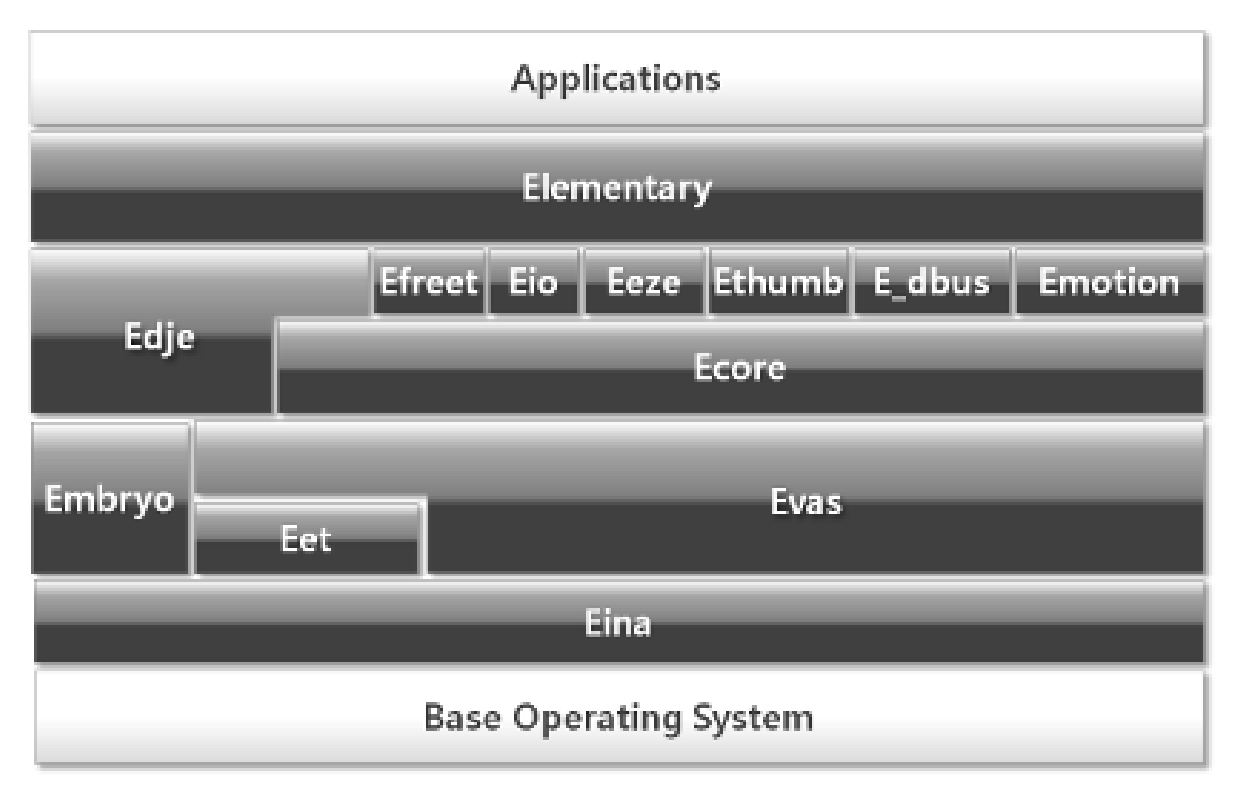
\includegraphics[width=8cm, height=5cm]{./eps/efl}
 \caption{EFL structure.}
 \label{fig:myfigure1}
\end{figurehere}

The \textit{Small} language, renamed Pawn \cite{pawnLang}, is an open source scripting language intended to be embeddable. It is a simple, typeless, 32-bit extension language with a C-like syntax. A source program is compiled to a binary file for optimal execution speed. The compiler outputs a \textit{P-code} (or bytecode) that subsequently runs on an abstract machine.\\
Embryo implements a subset of \textit{Pawn/Small} features as described in \cite{embyoLang}. In its most recent version (1.7.0), Embryo depends on another EFL library, named Eina \cite{einaLib}. Eina is a library that implements APIs for data types and provides some tools like opening shared libraries, errors management, type conversion and memory management. Although some of these features can be useful, we preferred to rely on an older version of Embryo (1.1.0) which is not depending on any other library, neither for the compiler, nor for the abstract machine.

%-----------------------------------------------------------------------------
\subsection{ChibiOS/RT}

ChibiOS/RT is a RTOS designed for embedded applications on 8, 16 and 32 bits microcontrollers focused on size and execution efficiency \cite{wikiChibi}. The kernel size can range from a minimum of 1.2Kbytes up to a maximum of 5.5Kbytes  on a STM32 Cortex-M3 processor. The kernel is able to perform a Context Switch in 1.2 microseconds on a 72 MHz STM32.\\
ChibiOS/RT has also a lot features \cite{chibiHP} that simplify application development on embedded systems:

\begin{itemize}
\item Efficient and portable preemptive kernel,
\item Best in class context switch performance.
\item Static architecture, everything is statically allocated at compile time.
\item Dynamic extensions, dynamic objects are supported by an optional layer built on top of the static core.
\item Rich set of primitives: threads, virtual timers, semaphores, mutexes, condition variables, messages, mailboxes, event flags, queues.
\item HAL component supporting a variety of abstract device drivers
\end{itemize}

The current stable release of ChibiOS/RT is 2.4.2 and we worked on this one.


%-----------------------------------------------------------------------------
\subsection{Demoboard}

We decided to work with an ARM Cortex\texttrademark-M3 processor \cite{armcm3}, for its performance and for its wide range of interfaces and because it is one of the most used in industry applications. We selected a demoboard (see {\bf Figure \ref{fig:myfigure2}}) produced by Olimex \cite{olimex}, based on a \textit{STM32F107} processor \cite{stm32f107}.
Among other features, we mainly used the following components:

\begin{itemize}
\item 256 Kbyte Flash, 64 Kbyte RAM
\item 10 timers
\item 2 ADCs
\item JTAG connector with ARM 2x10 pin layout for programming/debugging
\item RS232
\item 2 user buttons
\item 2 status led 
\end{itemize}

\begin{figurehere}
 \centering
 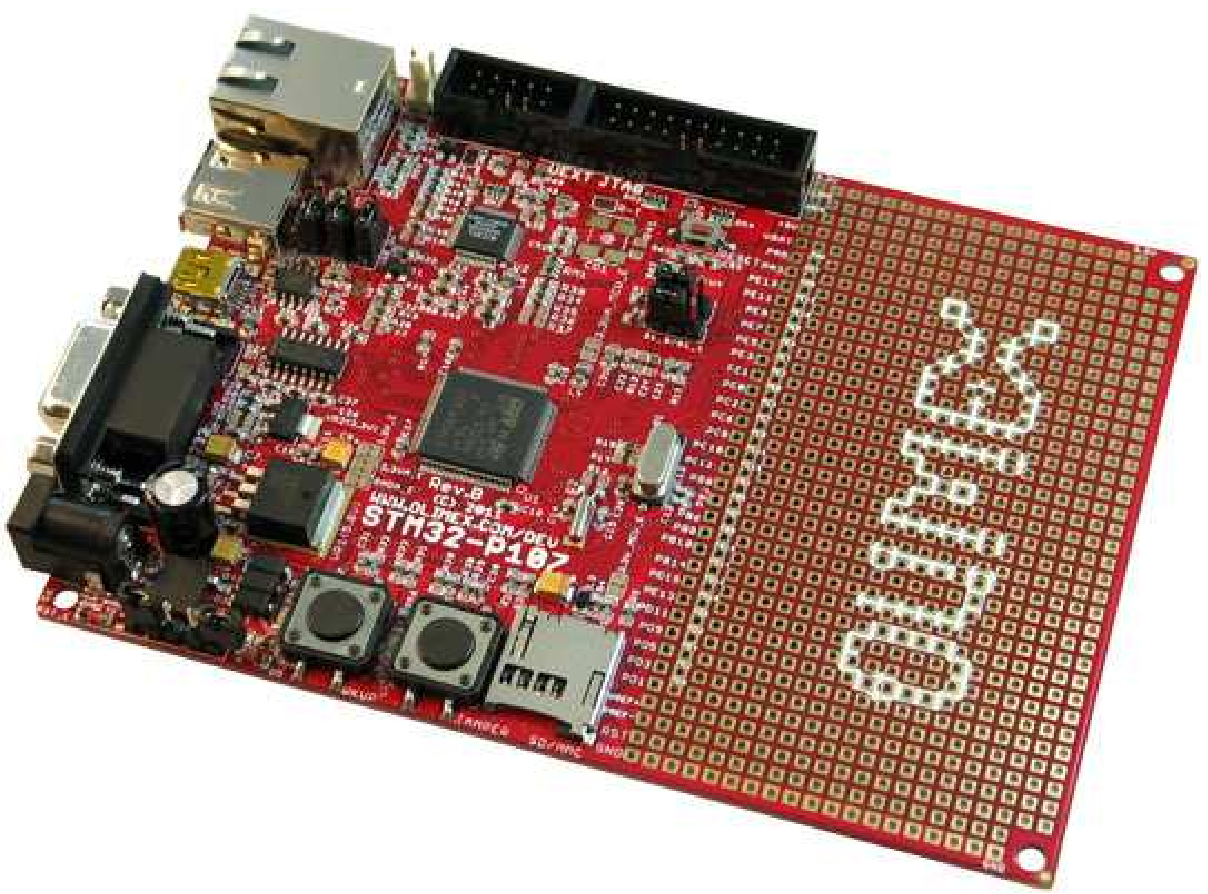
\includegraphics[width=8cm, height=5cm]{./eps/STM32P107}
 \caption{Olimex STM32P107 demoboard.}
 \label{fig:myfigure2}
\end{figurehere}

%-----------------------------------------------------------------------------
\subsection{Development and testing equipment}

The code has been written using the \textit{Eclipse CDT} IDE \cite{cdt}, and has been compiled using the CodeSourcery ARM EABI compiler, maintained by Mentor Graphics \cite{sourcery}.\\
In order to run and debug the program, we used the JTAG interface produced by Olimex (see {\bf Figure \ref{fig:myfigure3}}), which allows debug operations via ARM JTAG interface and communication via an RS232 Serial interface.

\begin{figurehere}
 \centering
 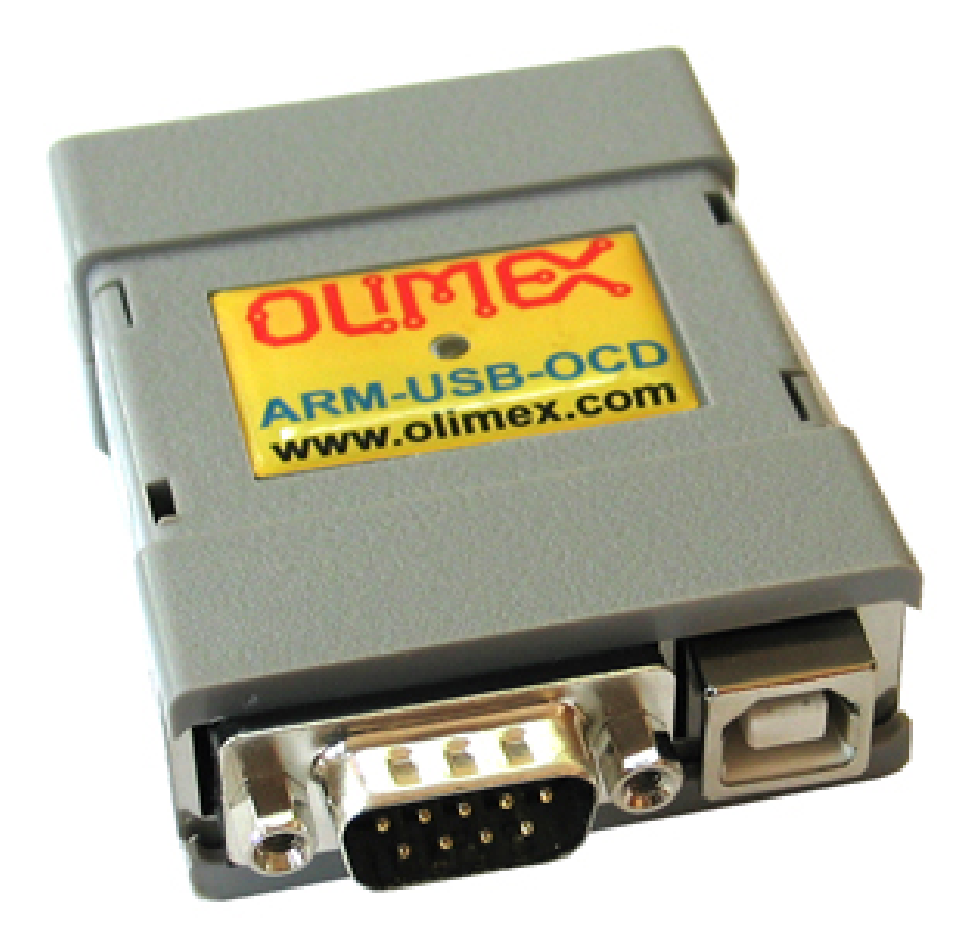
\includegraphics[width=6cm, height=6cm]{./eps/arm-usb-ocd}
 \caption{Olimex JTAG interface.}
 \label{fig:myfigure3}
\end{figurehere}

The setup operations followed instructions found here \cite{setup1} and here \cite{setup2}.


%%%%%%%%%%%%%%%%%%%%%%%%%%%%%%%%%%%%%%%%%%%%%%%%%%%%%%%%%%%%%%%%%%%%%%%%%%%%%
\section{Development}

In this section we describe the main phases of the development of the project.


%-----------------------------------------------------------------------------
\subsection{Project Structure}

The project structure is the following:
\newline

\dirtree{%
	.1 /\DTcomment{git root}.
	.2 ChibiOS-EmbrIO.
	.2 embryo.
	.3 embryo-cc\DTcomment{compiler}.
	.3 embryo-lib\DTcomment{abstract machine}.
	.3 embryo-sim\DTcomment{simulator}.
	.2 report.
	.1 ChibiOS/RT.
}
\bigskip
The project is managed by using a Git revision control system and is hosted on \url{http://code.google.com/p/chibios-embrio/}. ChibiOS/RT is mainly untouched and is out of revision control. The compiler and the abstract machine derive from Enlightenment code, while the simulator is a really small tool developed in order to test the basic functionalities of the abstract machine. The original Embryo project is managed by the \textit{GNU Automake} tool. In order to use different compilation parameters (the abstract machine can be compiled for ARM but also for a host pc), a new \texttt{Makefile} has been generated.

%-----------------------------------------------------------------------------
\subsection{Embryo Compiler}

The compiler underwent the least modifications. None of the components that build the bytecode has been touched. The original code is very Linux-oriented, looking for default paths like \texttt{/usr/bin} or looking into the \texttt{/proc} filesystem. As some of the development has been carried on in a Windows environment, the whole setup of the paths has been simplified.\\
The Embryo Abstract Machine allows the user to define his own \textit{native functions}, which extend the basic functionalities of a program and allow to reduce the code size. The Embryo compiler just needs to know the signature of the native functions; the user can include any \texttt{*.inc} files with the function signatures. The user needs only to indicate the directories where the compiler must search for the files. The source code is very similar to C:

\begin{lstlisting}[caption={include directives in Embryo}]
/* files with native functions to include */
#include <printXXX>
#include <embrio01>

\end{lstlisting}
We encountered some difficulties when looking for \texttt{*.inc} files and so we slightly modified the way Embryo compiler looks into the directories where the files are.\\
Finally we changed the command line arguments used to call \texttt{embryo\_cc}, using the conventions of \texttt{getoptlong.h}.
\bigskip
\lstset{language=bash}
\begin{lstlisting}[caption={Command line arguments}]
Usage:   embryo_cc -c  <filename> [options]

Options:
        -i  (--include) <name> path of include files
        -o  (--output) <name> base name of output file
        -S  (--size) <num>  stack/heap size in cells (default=4096, min=65)

        -h  (--help)  Display usage information
\end{lstlisting}


%-----------------------------------------------------------------------------
\subsection{Embryo Abstract Machine}

The Embryo Abstract Machine needed modifications in two areas: the definition of native functions and the memory management. Embryo gives the chance to define one's own functions and so we used it to call ChibiOS/RT functions within the Embryo environment. As we wanted to test the Abstract Machine also on a pc, we used the \texttt{\#define} directive to select the compilation environment.

\subsubsection{Native Functions}
\lstset{language=C}
\begin{lstlisting}[caption={Native function \textit{sleep}}]
Embryo_Cell
_embryo_sleep(Embryo_Program *ep, Embryo_Cell *params)
{
#ifdef _CHIBIOS_VM_
	chThdSleepMilliseconds(1000);
#else
	sleep(1);
#endif

	return 0;
}
\end{lstlisting}
\bigskip
The code above shows that under \texttt{\_CHIBIOS\_VM\_} we can call ChibiOS/RT functions.\newline
The following code shows the usage of the board serial port (called \texttt{SD3} in ChibiOS/RT), so that a string inside an Embryo VM can be directly displayed on a log terminal. While testing the functionalities, we simply print on \texttt{stdout}.

\begin{lstlisting}[caption={Native function \textit{print}}]
Embryo_Cell
_embryo_print(Embryo_Program *ep, Embryo_Cell *params)
{
	char *s;

	/* params[1] = str */
	if (params[0] != (1 * sizeof(Embryo_Cell))){
		return -1;
	}

	STRGET(ep, s, params[1]);
#ifdef _CHIBIOS_VM_
	chprintf((BaseChannel*)&SD3, "%s",s);
#else
	printf("Stringa: %s\n", s);
#endif
	return 0;
}
\end{lstlisting}

\subsubsection{Memory Management}
\label{sec:mm}
ChibiOS/RT has a static kernel, but offers different ways to manage memory for the applications \cite{chMem}:

\begin{itemize}
\item Core Memory Manager
\item Heap Allocator
\item Memory Pools
\end{itemize}

The \textit{core memory manager} is a simplified allocator that only allows to allocate memory blocks without the possibility to free them, it is meant to be a memory blocks provider for the other allocators.\newline
The \textit{heap allocator} implements a first-fit strategy to allocate chunks of memory. It is subject to fragmentation, and the allocation time is not constant. Its APIs are functionally equivalent to the usual C \texttt{malloc()} and \texttt{free()}.\newline
\textit{Memory pools} allow to allocate and free fixed size objects, in constant time and reliably (no fragmentation problems, thread safe...). Memory pools can grow in size if a suitable memory provider has been defined.
As we want the possibility to load, unload and change Virtual Machines at execution time, flexibility plays a key role in memory management. We needed to analyze how and where the Embryo Abstract Machine allocates and releases memory and translate the memory operations into the best suitable ChibiOS/RT APIs.\newline
\bigskip
We defined:

\begin{itemize}
\item an EmbrIO Memory Heap
\item a set of Memory Pools
\end{itemize}

We used the Heap for all the elements that are of unknown size at compile time (e.g. bytecode) while we defined different Memory Pools for every set of objects that can be allocated and freed. We defined the maximum number of Virtual Machines that can be run at the same time and allocated the corresponding pools (e.g. the \texttt{Embryo\_Program} structure, the Thread running the VM, the VM itself).
\smallskip
\begin{lstlisting}[caption={Memory Pools}]
// define the max number of virtual machines and programs
#define MAX_EMBRIO_VM_NUM 4
...
{
	/* init MP for thread used for VMs */
	chPoolInit( &THD_mp, THD_WA_SIZE(THD_STACK_SIZE), NULL);
...
	/* preallocate */
	for (i = 0; i < MAX_EMBRIO_VM_NUM; ++i) {
		chPoolFree(&THD_mp, thd_vm_wa_p[i]);
	}
...
	/* allocate a MP element to a Thread */
	thdp = chThdCreateFromMemoryPool( &THD_mp, prio, vm_thread, (void *)vm);

}
\end{lstlisting}

%-----------------------------------------------------------------------------
\subsection{Embryo Simulator}

A new component, although very simple, has been added to the original structure of the Embryo compiler and abstract machine, in order to test on a normal computer the basic functionalities. The abstract machine can be compiled to become a static library that can be linked to a testing program. The basic operations needed to use an Embryo program are described in \cite{embryoSite}.
\bigskip

\begin{lstlisting}[caption={Embryo basic simulator}]
int main(int argc,char *argv[]) {
	Embryo_Program* ep;
	Embryo_Status es;

	/* init Embryo */
	embryo_init();
	/* load program */
	ep = embryo_program_load(argv[1]);
	/* Starts a new VM session */
	embryo_program_vm_push(ep);
	/* run program from main function */
	es = embryo_program_run(ep, EMBRYO_FUNCTION_MAIN);
	/* at the end stop VM and free memory */
	embryo_program_free(ep);
	/* close Embryo */
	embryo_shutdown();
	return 0;
}

\end{lstlisting}

%-----------------------------------------------------------------------------
\subsection{ChibiOS-EmbrIO}
ChibiOS-EmbrIO is the core part of the program. It derived from demo code written in ChibiOS-2.4.2 and adapted to include all the functions and APIs to enable ChibiOS/RT subsystems and Embryo Abstract Machine.

\subsubsection{Configuration files}

ChibiOS/RT has a specific set of files used to define all the architecture (see {\bf Figure \ref{fig:myfigure4}}) \cite{chArch}:

\begin{itemize}
\item \texttt{chconf.h} defines Kernel parameters and options, such as system tick frequency, or IPC elements to be loaded.
\item \texttt{halconf.h} to define the high level Hardware Abstraction Layer (HAL) components. It allows to enable or disable the various device drivers for the application. The low level HAL is hardware specific and is part of the ChibiOS/RT source tree.
\item \texttt{mcuconf.h} to define driver configurations and it is hardware specific. In our case \textit{STM32F1xx} definitions were used.
\end{itemize}

\begin{figurehere}
 \centering
 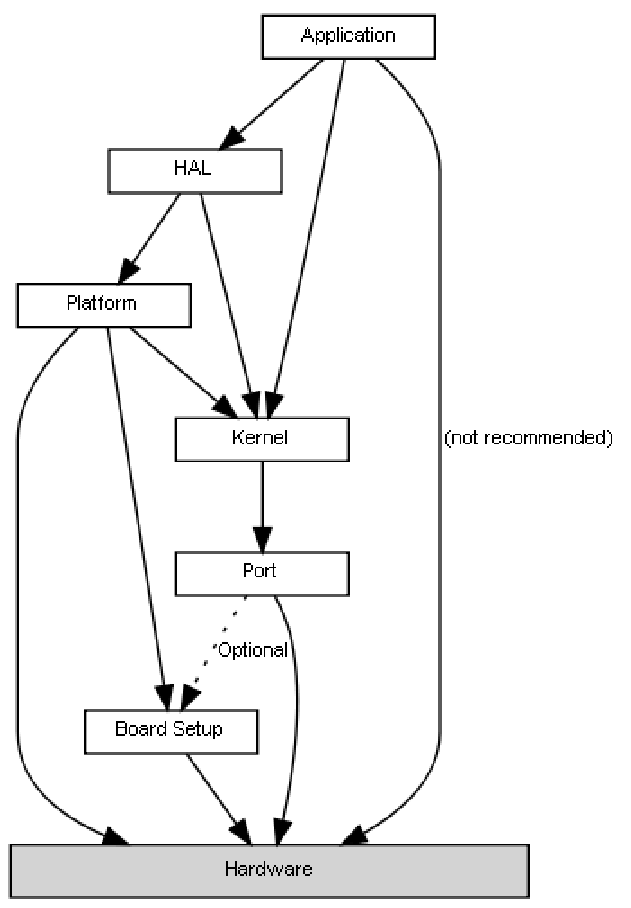
\includegraphics[width=8cm, height=9cm]{./eps/architecture}
 \caption{ChibiOS/RT architecture.}
 \label{fig:myfigure4}
\end{figurehere}

As our demoboard is already part of the ones defined in ChibiOS/RT, it was quite simple to reuse and adapt all the configuration files to our needs.

\subsubsection{Application code}

The application code takes care of setting up the system and then running the Embryo Virtual Machines. The setup phase initializes all the ChibiOS/RT Kernel and HAL components, and then initializes all the Embryo components that need some ChibiOS/RT API, e.g. Memory Management (see \ref{sec:mm}).\newline
ChibiOS-EmbrIO is organized with and \textit{Virtual Machine Manager} and multiple \textit{Virtual Machines}, from zero up to a maximum number defined at compile time. Each Virtual Machine is represented by a C \texttt{struct} with the following fields:

\begin{lstlisting}[caption={EmbrIO VM}]
struct EmbrioVM {
	/* state of the VM (running, etc.)*/
	EmbrioVMstate_t	state;
	/* thread running the VM */
	Thread			*tp;
	/* program to be executed */
	Embryo_Program	*ep;
	/* function pointer to callback */
	Embrio_hook		hook;
	/* callback parameters */
	int				hook_params;
	/* next VM in linked list of VMs */
	EmbrioVM		*vm_next;
};

\end{lstlisting}

\begin{itemize}
\item \textit{state} represent the current condition of the machine: running, stopped, waiting, etc.
\item \textit{tp} is a pointer to the thread that runs the VM on ChibiOS/RT
\item \textit{ep} is a pointer to the Embryo program to be executed
\item \textit{hook} is a function pointer to a callback that can be defined at runtime
\item \textit{hook\_params} is a parameter that can be passed to the callback
\item \textit{vm\_next} is a pointer to the next VM in the chain of VM created.
\end{itemize}


The Virtual Machine Manager, at the present state of development, is a simple \texttt{struct} that maintains a status, the number of VMs and a pointer to the first of them.

\begin{lstlisting}[caption={EmbrIO VM}]
typedef struct {
	EmbrioVMMstate_t	state;
	uint8_t				vm_count;
	EmbrioVM			*vm_first;
} EmbrioVMManager;
\end{lstlisting}



After initializing ChibiOS/RT, two threads are spawned by default \cite{chThd}:
\begin{itemize}
\item \textbf{Idle thread}. This thread has the lowest priority in the system so it runs only when the other threads in the system are sleeping. This thread switches the system in a low power mode and does nothing else.
\item \textbf{Main thread}. This thread executes the \texttt{main()} function at startup. It is from the main thread that the other threads running the VM are created.
\end{itemize}

In ChibiOS-EmbrIO the main thread initializes all the needed timers (GPT: General Purpose Timer), used either by different drivers (e.g. SPI) or to call cyclic routines and configures all the external interrupts (EXT: generic EXTernal driver) and subsequent callbacks (e.g. what to do when a button is pressed ), and then spawns a thread for each Embryo Virtual Machine.
\bigskip
\begin{lstlisting}[caption={EmbrIO VM start}]
/* allocate Memory Pool element for first VM */
vm[0] = (EmbrioVM*)chPoolAlloc(&EVM_mp);

/* Pool allocated */
if(vm[0] != NULL){
	/* insert VM in linked list of VMs */
	embrioVMMinsert(vm_man, vm[0]);
	/* load Embryo Program */
	vm[0]->ep = embryo_program_load_local(...);
}

/* program loaded correctly */
if(vm[0]->ep != NULL){
	/* set initial callback */
	vm[0]->hook = NULL;
	/* spawn and start VM thread */
	vm[0]->tp = vmStart(vm[0], NORMALPRIO, "VM0");
}
\end{lstlisting}
\bigskip
After initialization, every Virtual Machine is running, and the execution depends on the following elements:
\begin{itemize}
\item \textit{Embryo bytecode}: the operations that are coded in each Embryo Program,
\item \textit{Native Functions}: these are the connection points between Embryo and ChibiOS/RT, their implementation allow to use ChibiOS/RT services inside an Embryo VM,
\item \textit{Drivers}: which drivers that are enabled and what functions are called as a callback,
\item \textit{Callbacks}: which Embryo functions are invoked by the callback.
\end{itemize}

As the overall behavior strongly depends on the elements above, for that reason some tests have been conducted to implement few first simple functionalities in order to analyze the system performances. In the following section we describe the setup and the tests that we carried on.


%%%%%%%%%%%%%%%%%%%%%%%%%%%%%%%%%%%%%%%%%%%%%%%%%%%%%%%%%%%%%%%%%%%%%%%%%%%%%
\section{Application Code}

\subsection{Embryo Code}

We decided to implement to Virtual Machines with similar source code. As described in \cite{pawnGuide}, Pawn and also Embryo allow an \textit{event-driven} programming model. The main advantage of this model consists in building reactive programs, which respond to multiple events. The program has more than one entry point: while the \texttt{main} function runs immediately after you start the script and it runs only once, every function whose name begins with @ runs every time it is called. We coded two similar programs to be executed on two different VMs. The following code is an example:
\bigskip
\begin{lstlisting}[caption={EmbrIO first VM}]
#include <printXXX>
#include <embrio01>
/** global state variable */
new state = 0

/** event associated to first timer:
 *  VM toggles first led of demoboard if UP*/
@eventGPT1()
{
	if(state == 1){
		toggleLED1()
	}
}

/** event associated to second timer:
 *  VM reads samples from ADC if UP */
@eventGPT2()
{
	if(state == 1){
		readADC1()
	}
}

/** event associated to external interrupt
 *  the VM toggles state (UP or DOWN) and prints
 *  the status on serial port */
@eventEXTI1()
{
	if(state == 0){
		state = 1
		printXXX("\r\nVM 0 UP\r\n")
	}else{
		state = 0
		printXXX("\r\nVM 0 DOWN\r\n")
	}
}
/** application entry point:
 *  sets a 'state' variable to 1 (UP)
 * and prints on the serial port */
main()
{
	state = 1
    printXXX("\r\nVM 0 UP\r\n")
}
\end{lstlisting}

\subsection{Embryo Compile and Load}

The code has then been compiled with the following command string:
\medskip
\lstset{language=bash}
\begin{lstlisting}[caption={compile command}]
embryo-cc -c vm0.p -S 128
\end{lstlisting}
\medskip
The execution outputs a \texttt{vm0.eaf} file (Embryo Assembly File). It is important to note that, in order to reduce stack size and overall program size, it is mandatory to use the \texttt{-S} option using the least feasible stack/heap size, otherwise \texttt{Embryo\_Program} requires too many Kbytes of memory.
Further development in ChibiOS-EmbrIO will allow assembly code to be loaded into memory by using some communication interface (e.g. Serial RS232, CAN, etc...). At present state, no particular interface is fully functional and so we decided to load the assembly code together with the rest, linking it at compile time. We first used the following command:
\medskip
\lstset{language=bash}
\begin{lstlisting}[caption={object code command}]
arm-none-eabi-objcopy -I binary -O elf32-littlearm -B arm vm0.eaf vm0_eaf.o
\end{lstlisting}
\medskip
By linking the \texttt{vm0\_eaf.o} together with the rest of object files, we can use the following \texttt{extern} variables to access the code, which will be loaded in RAM.
\medskip
\lstset{language=C}
\begin{lstlisting}[caption={code location variables}]
/* VM0 code references */
extern unsigned char _binary_vm0_eaf_start;
extern unsigned char _binary_vm0_eaf_end;
extern unsigned char _binary_vm0_eaf_size;
\end{lstlisting}
\medskip
When loading a new program, we refer to the variables above to access the data.
\medskip
\lstset{language=C}
\begin{lstlisting}[caption={Program load}]
/* VM0 load from memory */
vm[0]->ep = embryo_program_load_local(
				&_binary_vm0_eaf_start,
				&_binary_vm0_eaf_end,
				 &_binary_vm0_eaf_size,
				/* log options */
				(BaseChannel*)&SD3, TRUE);
\end{lstlisting}
\medskip
Upon successful load, the program can be executed by an Embryo Virtual Machine.

\subsection{Drivers and Callbacks}
We decided to implement the following drivers and callbacks:

\begin{itemize}
\item \textit{TIM1}: timer 1 gives the \textit{heartbeat} of the Virtual Machine, if it is in UP state makes the led  blink. Each Virtual Machine makes a different led blink. The function name is the same (\textit{@eventGPT1}) for every VM, but the code is different.
\item \textit{TIM2}: timer 2 triggers an ADC conversion: the first VM has a function named (\textit{@eventGPT2}) that is used to read the ADC samples and to print data on serial port. The function operates only when the Virtual Machine is UP.
\item \textit{TIM3}: timer 3 triggers a SPI read: the second VM has a function named (\textit{@eventGPT3}) that is used to read the SPI data from a sensor connected to the board and to print the data on serial port. The function operates only when the Virtual Machine is UP.
\item \texttt{EXTI1}: the external interrupt driver can be used to connect different interrupt sources to different callbacks. In our case we connected a callback to the first user button and another callback to the second user button. The first VM defines a function named \texttt{@eventEXTI1} that toggles its state and the second VM has a similar function named \texttt{@eventEXTI2}.
\end{itemize}

\subsection{Dispatch of Callbacks}
In this first implementation of Embryo Virtual Machines on ChibiOS/RT, we decided not to implement \textit{argument passing} to and from Embryo functions, leaving the implementations of \textit{hook} and \textit{hook\_params} to further development.\newline
Each callback simply needs to call an event function in a program without arguments, and accomplishes this task by looking for the function in each machine. If the function is part of the code (i.e. it can be run on the VM), the Embryo function \texttt{embryo\_function\_find} does the work for us: it returns a specific value (\texttt{EMBRYO\_FUNCTION\_NONE}) if there is no corresponding function or a number that can be used to identify and execute the function itself.\newline
The following code illustrates the operation described here:
\medskip
\lstset{language=C}
\begin{lstlisting}[caption={Callback looking for a function in VMs}]
/* TIM1 callback */
void gpt1cb(GPTDriver *gptp) {

	EmbrioVM *vm_tmp;
	Embryo_Function ef;
	
	/* the first VM is pointed by VM Manager */
	vm_tmp = vm_man->vm_first;
	
	/* we look into all VMs */
	while(vm_tmp != NULL){
		
		/* function that tells if a function is in the VM */
		ef = embryo_program_function_find(vm_tmp->ep, "@eventGPT1");
		
		/* if available we send a message to thread */
		if(ef != EMBRYO_FUNCTION_NONE){
			chMsgSend(vm_tmp->tp,(msg_t)ef);
		}
		
		/* we go to next VM */
		vm_tmp = vm_tmp->vm_next;
	}
}
\end{lstlisting}
\medskip
In the example above, a timer event triggers the callback function (named \texttt{gpt1cb}), which looks for a specific function (here \texttt{@eventGPT1}) and, if it is found, sends a message to the corresponding thread. Note that different VMs can implement the same function in different ways, allowing some flexibility: in our case, with the same callback, one VM makes the green led blink and the other vM makes yellow led blink.\newline
The \textit{EmbrIO\_VM} \texttt{struct} carries all the necessary information (i.e. pointer to the program, pointer to the thread, ...) to perform the operation.\newline
\medskip
When a Virtual Machine thread is spawned, it loads the code, then executes the main function and finally enters an infinite loop waiting for messages. Note that a callback sends a different message to each thread that is involved, and the message carries the value of the function to be executed, coded as a \texttt{Embryo\_Function} parameter. When the message arrives, the thread wakes up and executes the corresponding function. The following code illustrates the operations described above:
\medskip
\lstset{language=C}
\begin{lstlisting}[caption={Callback looking for a function in VMs}]
{
	/* load Embryo Program */
	embryo_program_vm_push(vmp->ep);
	
	/* run main function */
	es = embryo_program_run(vmp, EMBRYO_FUNCTION_MAIN);
	
	/* enter infinite loop */
	while(TRUE){
		/* wait for message */
		tp = chMsgWait();
		
		/* get message = function to be executed */
		ef = (Embryo_Function)chMsgGet(tp);
		
		/* acknowledge sending thread */
		chMsgRelease(tp, RDY_OK);
		
		/* execute function */
		es = embryo_program_run(vmp, ef);
	}
}
\end{lstlisting}\medskip

The code above is the same for all the threads that are spawned. The only difference consists in the Embryo code that is loaded when the Virtual Machine is created.

%%%%%%%%%%%%%%%%%%%%%%%%%%%%%%%%%%%%%%%%%%%%%%%%%%%%%%%%%%%%%%%%%%%%%%%%%%%%%
\section{Tests}

We tested the application in two different phases. At first we analyzed the behavior of the system itself (see setup in Figure \ref{fig:myfigure5}):

\begin{itemize}
\item 2 Virtual Machines
\item 3 GPT callbacks
\item 2 EXT interrupt callbacks connected to buttons
\item mock native functions for ADC and SPI callbacks (substituted with serial port log)
\end{itemize}

Within this environment we verified that the system worked as expected: with the two buttons enabling and disabling the VMs.\newline
We tried changing the timers frequency and verified that the system continued working.
In a subsequent phase we started configuring the \textit{SPI} and \textit{ADC} HAL of ChibiOS/RT, to be able to read two different temperature sensors:

\begin{itemize}
\item a 5k$ \Omega $ NTC thermistor \cite{wikiTh} with a simple conditioning circuit \cite{embTh}.
\item a DS18B20 SPI temperature sensor with a connection scheme similar to the one used for an Arduino platform and described in \cite{spiArd}.
\end{itemize}

We used port C pins 10 to 12 to connect SPI sensor.


%%%%%%%%%%%%%%%%%%%%%%%%%%%%%%%%%%%%%%%%%%%%%%%%%%%%%%%%%%%%%%%%%%%%%%%%%%%%%
\section{Conclusions}

The main target of the project was to make Embryo and ChibiOS/RT work together, allowing Embryo programs run on Abstract Machines in a ChibiOS/RT environment. We saw that this kind of setup is feasible and promising in a lot of applications.\newline
Further development is still needed to complete some features and to extend the functionalities of ChibiOS-EmbrIO. In particular we cite:

\begin{itemize}
\item Load Embryo programs at runtime, using some communication interface (e.g. CAN).
\item Implement more native functions in order to use as many ChibiOS/RT services as possible, making ChibiOS/RT and Embryo more deeply connected. As a result, much more degrees of freedom will be available when writing Embryo programs.
\item Allow the use of \textit{argument passing} when calling Embryo function or use return values.
\item Complete the code of the Virtual Machine Manager, for example making it the central component that manages all the Virtual Machines, for example by using the \textit{queue} ChibiOS/RT service from external interrupts to the manager and messages from the manager to the VMs.
\item extend some Embryo functionalities (e.g. \textit{string} usage or \textit{Float} operations) if interesting for some applications.
\end{itemize}

Further analysis of the performances is also needed. In particular we cite:

\begin{itemize}
\item Analyze the optimal size of Embryo Programs, limiting stack/heap size without worsening Virtual Machine performances.
\item Measure execution time, in order to determine how fast we can execute VMs and so update data (this can be really interesting if applied to controllers). On the other hand, it can be interesting to determine if the message passing environment reaches a critical level for performances.
\item Evaluate if it is possible to optimize memory usage: for example when loading an Embryo program.
\end{itemize}

As a final remark we can state that ChibiOS-EmbrIO can have very interesting further development.

\begin{figure*}[t]
	\centering
	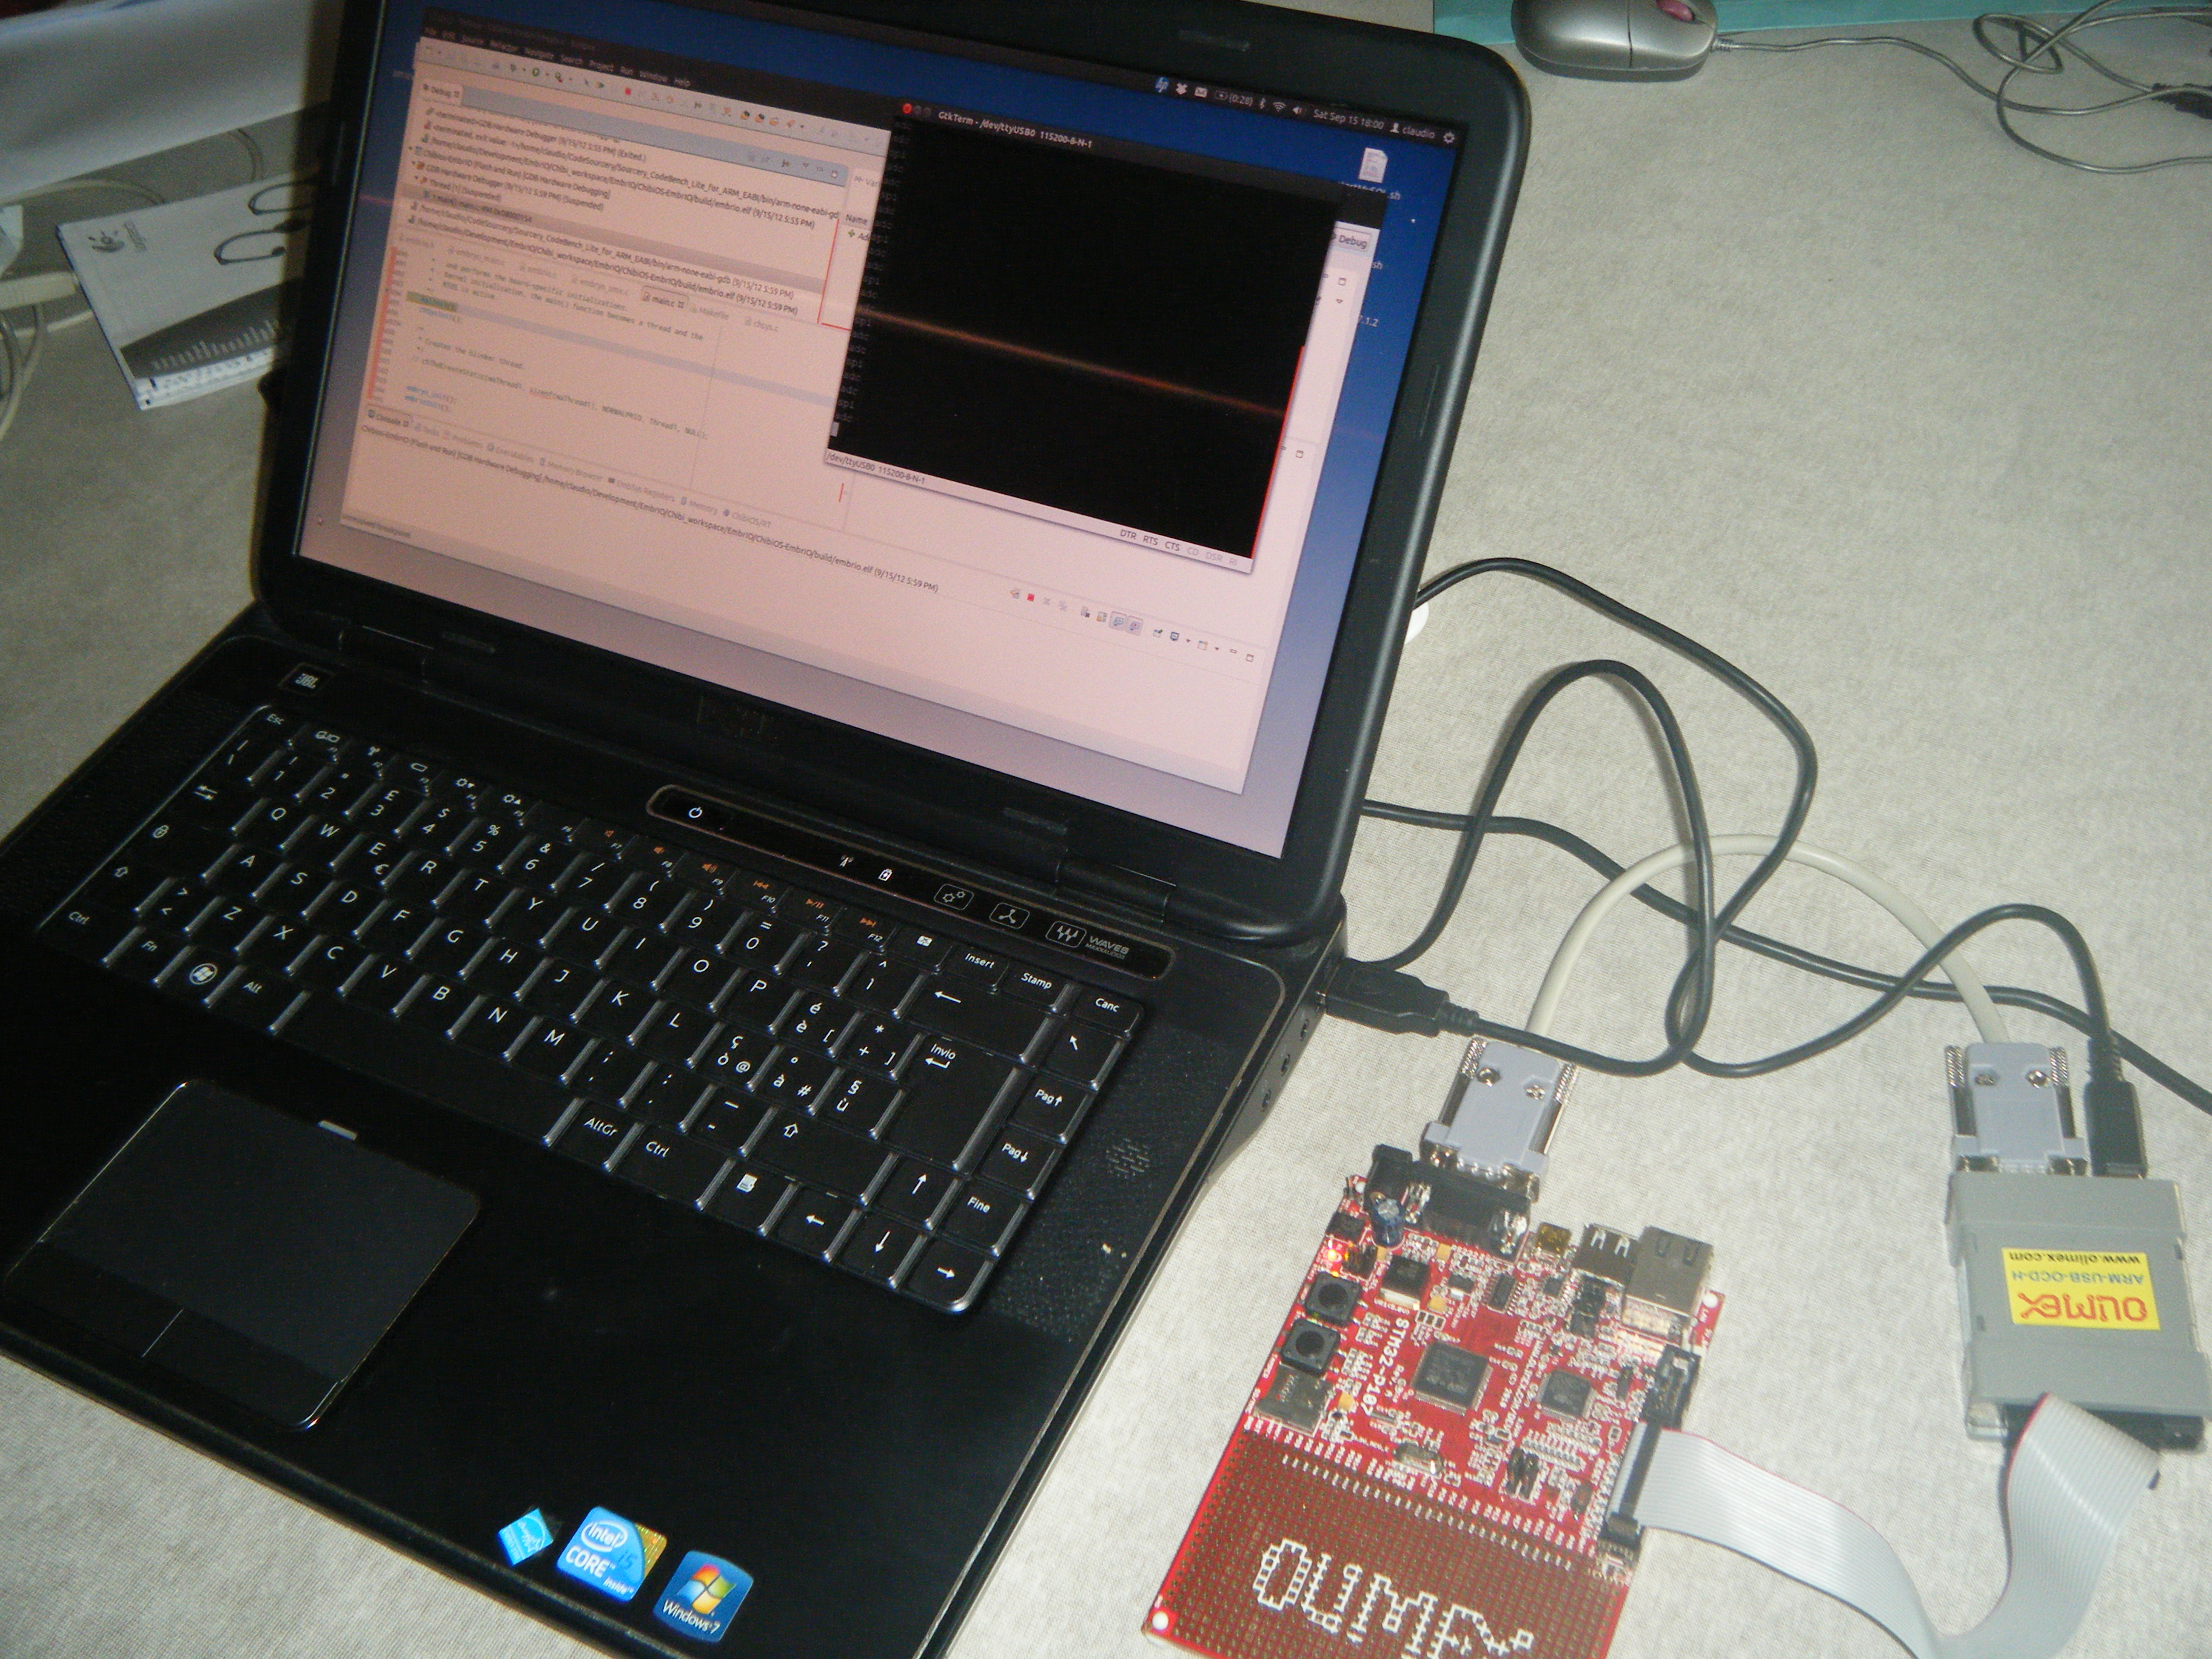
\includegraphics[width=16cm, height=12cm]{./eps/DSCF2211}
	\caption{Application and Hardware setup.}
	\label{fig:myfigure5}
\end{figure*}

% We suggest the use of JabRef for editing your bibliography file (Report.bib)
\bibliographystyle{splncs}
%\bibliographystyle{plainnat}
\bibliography{Report}

\end{multicols}
\end{document}
